\documentclass[10pt]{book}
%\documentclass[10pt, draft]{book}
\usepackage[nonumber]{cuisine}
%\usepackage[loose]{units}
\usepackage{units}
\usepackage{url}
%\usepackage{path}
\usepackage{graphicx}
\usepackage{layout}
\usepackage{caption}
\usepackage{makeidx}
\usepackage{titlesec}
\usepackage{hyperref}
\hypersetup{
  colorlinks=true, %set true if you want colored links
  linktoc=all,     %set to all if you want both sections and subsections linked
  linkcolor=blue,  %choose some color if you want links to stand out
  }
%\RecipeWidths{\textwidth}{0.01\textwidth}{0.2\textwidth}{0.25\textwidth}{0.09\textwidth}{0.08\textwidth}
% total, recipe #, servings, ingredients, quantity, units
\renewcommand*{\recipetitlefont}{\large\bfseries\sffamily}
%\renewcommand*{\recipetex\titlefont}{\large\bfseries\sffamily}
\renewcommand*{\recipequantityfont}{\sffamily\bfseries}
%\renewcommand*{\recipequantityfont}{\sffamily}
\renewcommand*{\recipeunitfont}{\sffamily}
\renewcommand*{\recipeingredientfont}{\sffamily}
\renewcommand*{\recipefreeformfont}{\itshape}
\makeindex
\newcommand{\jalapeno}{\ }
\newcommand{\jalapenos}{jalape\~{n}os\ }
\newcommand{\apf}{all purpose flour}
\newcommand{\bp}{baking powder}
\newcommand{\bs}{baking soda}
\newcommand{\ws}{Worcestershire sauce}
\newcommand{\tm}{\textsuperscript{\texttrademark}}

\titleformat{\chapter}{\bfseries\Huge\itshape}{}{0.5ex}{}{}
\newcommand{\mychapter}[1]{
  %\setcounter{chapter}{2}
  %\setcounter{section}{0}
  \chapter{#1}
  %\addcontentsline{toc}{chapter}{#1}
  }
\newcommand{\mysection}[1]{
  %\setcounter{section}{#1}
  \section*{#1}
  \addcontentsline{toc}{section}{#1}
  }
\newcommand{\mysubsection}[1]{
  %\setcounter{section}{#1}
  \subsection*{#1}
  \addcontentsline{toc}{subsection}{#1}
  }
\begin{document}
%\layout
\frontmatter
\begin{titlepage}
\vspace*{1.5in}
\begin{center}
\resizebox{\linewidth}{!}{\textbf{Younkin Family Cookbook}}\\
\vspace{1em}
\large{\itshape First Edition, March 2017; Updated, June 2024}\\
\vspace*{2em}
\Large{\slshape Julie \& Samuel Younkin}\\
\vspace*{0.5em}
\Large{\slshape Sarah \& Judd Goldberg}\\
\vspace*{0.5em}
\Large{\slshape Linda \& Steven Younkin}\\
%\vspace*{1in}
%\subtitle{
%\author{Sam \& Julie Younkin}
%\date{2013}
%\maketitle

% Upper part of the page
%\textsc{\LARGE University of Beer}\\[1.5cm]
%\textsc{\Large Final year project}\\[0.5cm]
% Title
%{ \huge \bfseries Lager brewing techniques}\\[0.4cm]
% Author and supervisor
%% \begin{minipage}{0.4\textwidth}
%% \begin{flushleft} \large
%% \emph{Author:}\\
%% John \textsc{Smith}
%% \end{flushleft}
%% \end{minipage}
%% \begin{minipage}{0.4\textwidth}
%% \begin{flushright} \large
%% \emph{Supervisor:} \\
%% Dr.\string~/Mark \textsc{Brown}
%% \end{flushright}
%% \end{minipage}

%% \vfill

%% % Bottom of the page
%% {\large \today}

\end{center}

\end{titlepage}

\cleardoublepage
Lorem ipsum dolor sit amet, consectetur adipiscing elit. Donec sed felis purus, ac dictum nunc. In ultricies ipsum dui, eget molestie felis. Pellentesque habitant morbi tristique senectus et netus et malesuada fames ac turpis egestas. Fusce mauris libero, aliquam a sollicitudin posuere, rhoncus sed odio. In ut nulla erat, eget pulvinar enim. Morbi dignissim fringilla fringilla. Aenean arcu turpis, mollis non auctor ac, adipiscing eu est.

Ut risus justo, tincidunt vel volutpat sollicitudin, pharetra sit amet libero. Suspendisse auctor magna quis diam ultrices gravida. Vestibulum vitae tortor lacus. Donec elit sem, interdum id lobortis non, accumsan vel odio. Integer at neque congue dolor malesuada lacinia accumsan at libero. Morbi porttitor posuere metus vel varius. Phasellus convallis feugiat viverra. Phasellus ut dolor et ante semper congue ut in enim. Ut auctor purus nec lectus iaculis tempus. Maecenas fringilla commodo dui eu tincidunt. Proin pretium, erat non ornare cursus, massa velit cursus tortor, semper ullamcorper risus enim facilisis magna. Sed lobortis sollicitudin lorem at egestas. Cras sed ante ante, et sollicitudin lectus. Proin vitae euismod est.

Cras semper purus euismod tellus viverra et tincidunt nisi consectetur. Cras faucibus, massa eget euismod volutpat, tellus magna rutrum massa, eget tristique nisi augue non ante. Aenean commodo purus vel magna molestie vitae aliquet neque tincidunt. Nulla facilisi. Etiam id quam id lacus congue ullamcorper ut non nisi. Nullam faucibus feugiat fringilla. Suspendisse at dui neque. Morbi sed mi erat, vitae adipiscing velit. Proin massa nisl, vestibulum id pulvinar sit amet, condimentum id tellus. Ut tempus, massa ac pharetra fermentum, elit magna ultrices enim, et vulputate elit nulla sit amet dui. Morbi eget dictum magna. Sed commodo laoreet enim, nec ultrices tortor pharetra ut. Quisque volutpat eros malesuada quam convallis pretium. Sed vitae nulla nunc, a condimentum ipsum.

Nulla in nunc non lectus gravida fringilla. Morbi et lectus vitae tortor adipiscing iaculis. Nunc ullamcorper molestie arcu quis imperdiet. Pellentesque nec erat dui. Pellentesque habitant morbi tristique senectus et netus et malesuada fames ac turpis egestas. Fusce sed pellentesque nisl. Sed sagittis magna vitae lacus commodo et placerat ipsum porta. Phasellus interdum fermentum nunc sit amet imperdiet. Vestibulum nec massa lorem. In vehicula, risus vel elementum consectetur, odio lorem aliquam sem, dignissim sodales dui mauris posuere libero. Phasellus vel molestie dui. Nulla faucibus fringilla lorem, laoreet tristique purus egestas non.

\begin{figure}[t]
\begin{center}
\includegraphics[width=0.8\textwidth]{/home/sgy/Dropbox/cookbook/figures/butternut}
\end{center}
\caption*{Our babies.}
\end{figure}


%% We have collected some of our favorite recipes from throughout the years.  Chapter \ref{chapter1} contains some of our family favorites, and Chapter \ref{chapter2} is devoted to our holiday dishes.   Lastly, Chapter \ref{chapter4} contains miscellaneous recipes that have previosly been typest with \LaTeX, and is thereore named ``The Rest.''

%% Some recipes have been handed down through the years, while others have bees ripped right from the pages of \textit{Joy of Cooking}.  We tried to attribute the recipe to its source when possible.  We hope you will be loving this book!

\begin{figure}[b]
\begin{center}
  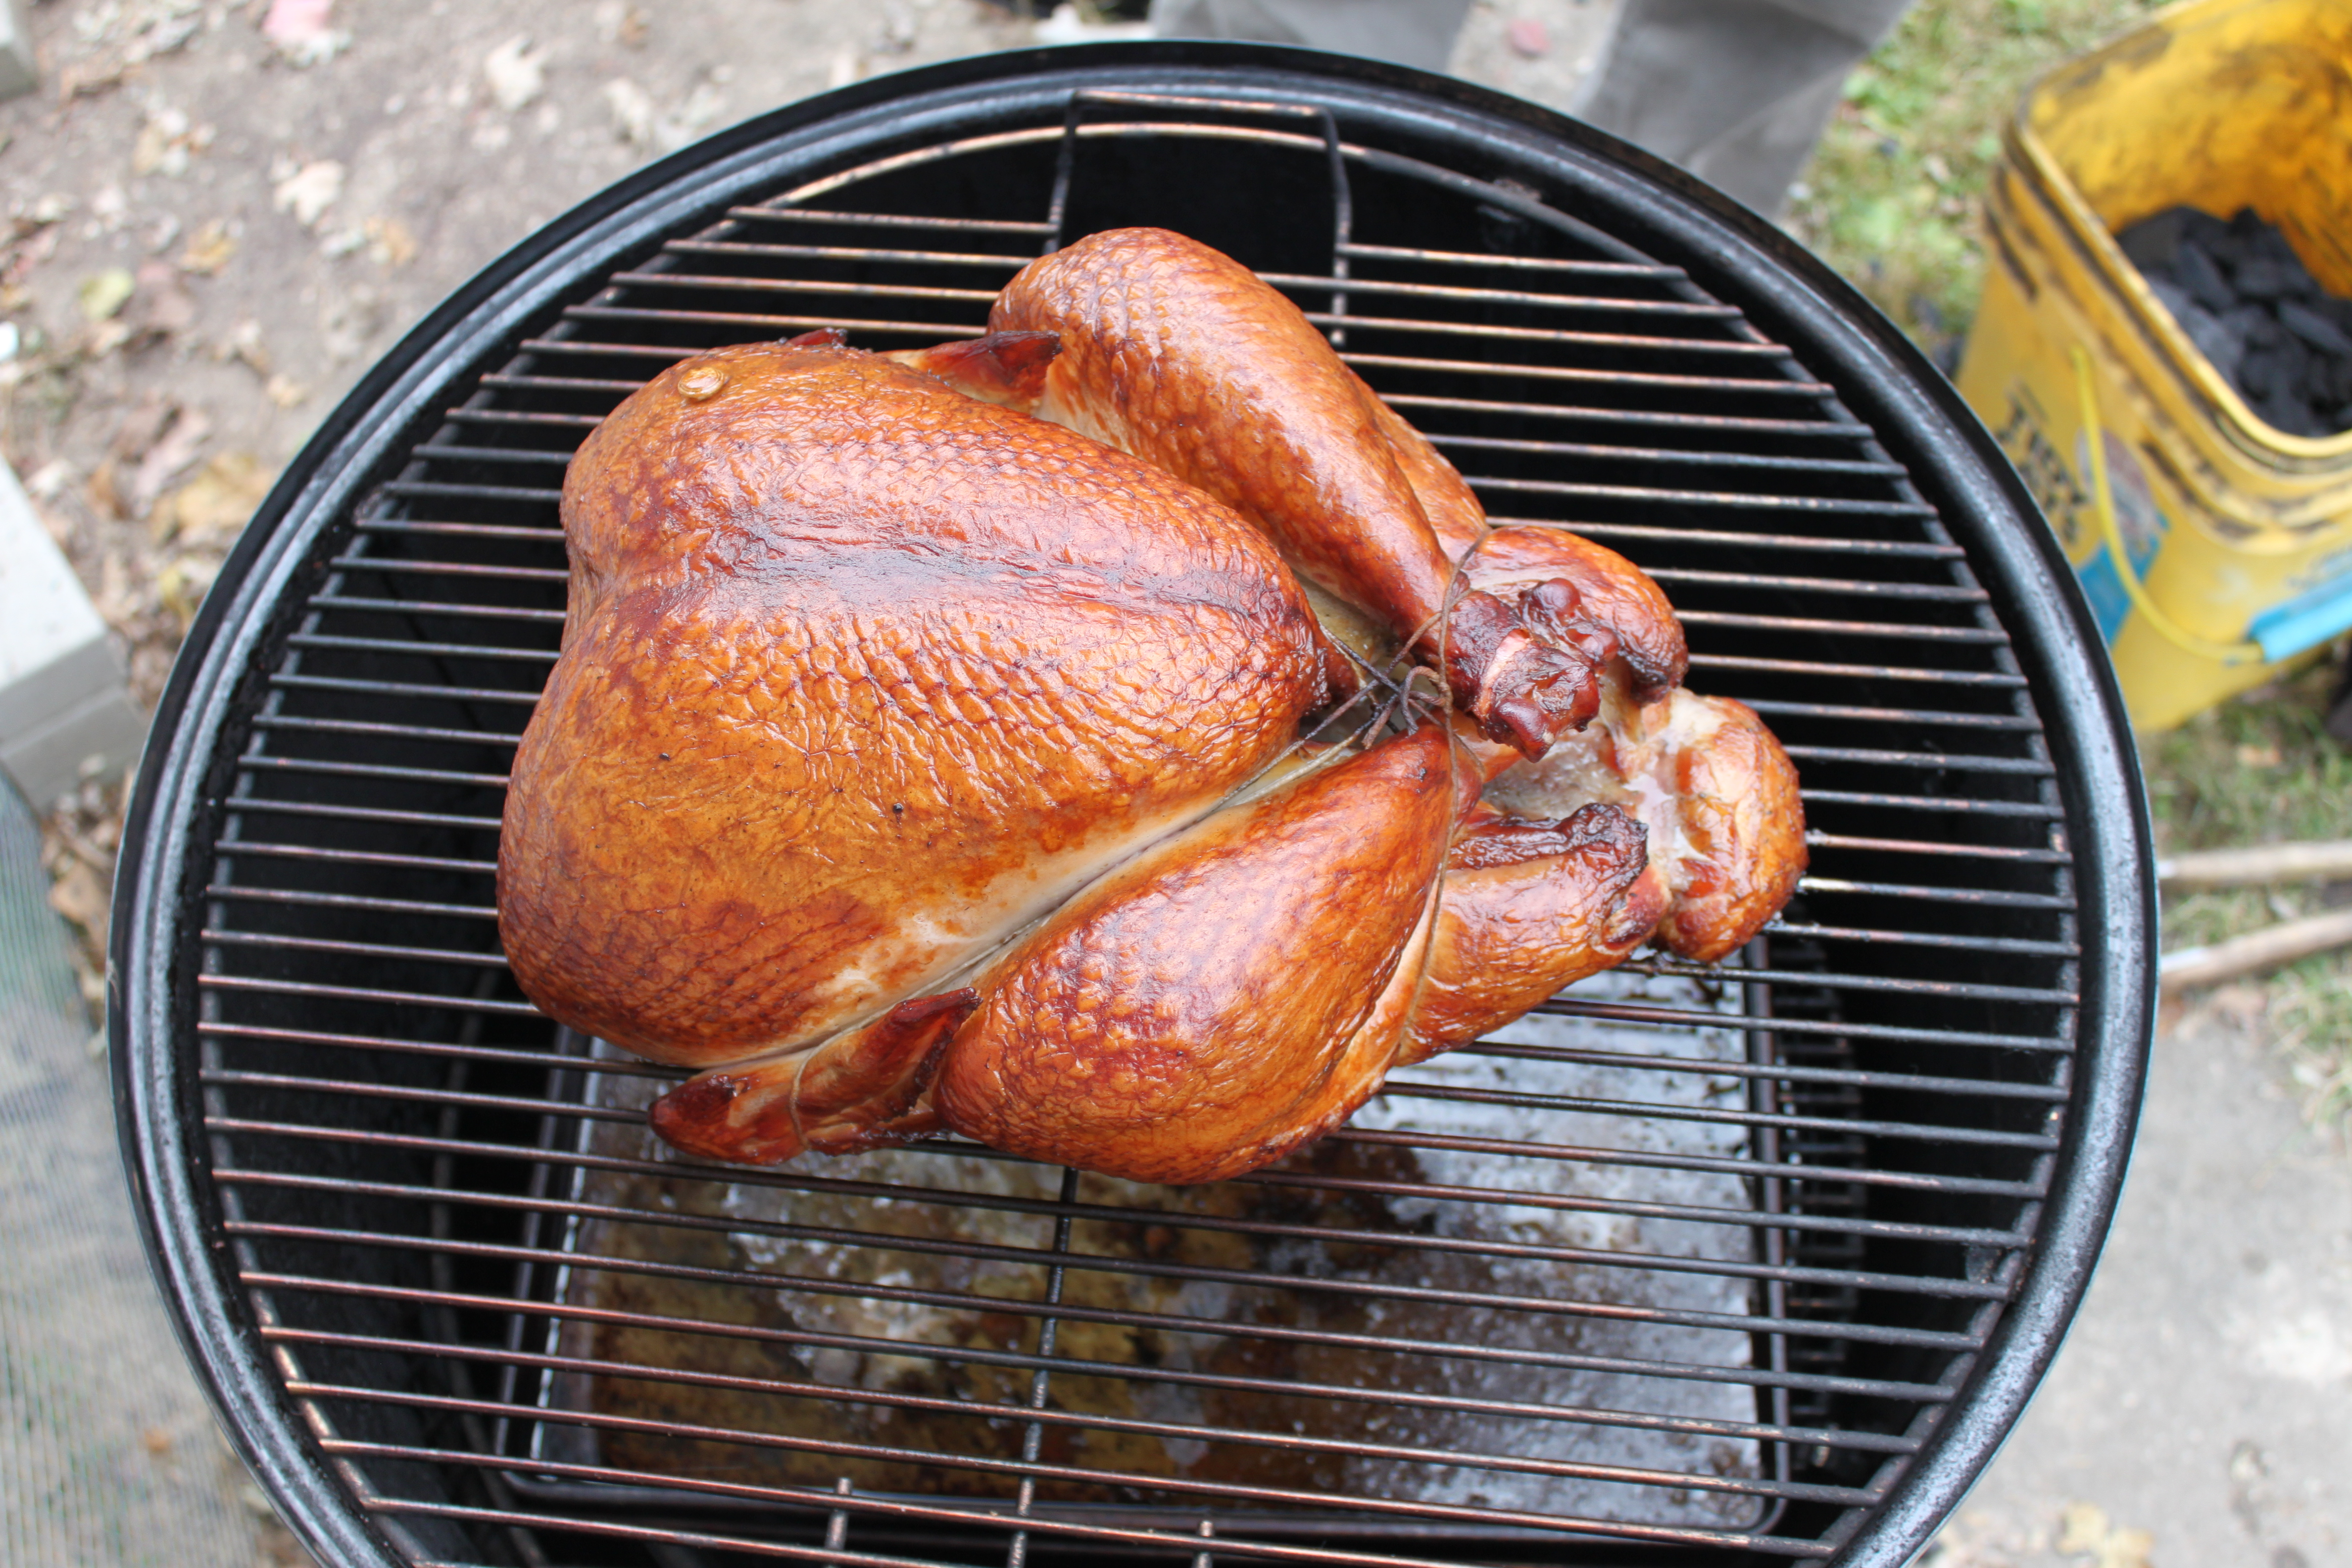
\includegraphics[width=0.8\textwidth]{./../figures/turkey}
  \includegraphics[width=0.8\textwidth]{./../figures/butternut}
\end{center}
%%\caption*{Butternut squash grown in Baltimore, Maryland (201?)}
\end{figure}
\tableofcontents
\mainmatter
\mychapter{Madison}
\mysection{Main Dish}\label{maincourse}
\index{Chili!Steve's}
\begin{recipe}{Steve's Chili}{\unit[6]{servings}}{\unit[90]{minutes}}
\freeform This recipe is from Steve Younkin. 
\ing[1]{}{onion, chopped}
\ing[2]{tbsp}{olive oil}
\ing[1]{lb}{ground turkey, preferably turkey breast}
\ing[5]{tbsp}{chili powder (Steve prefers Spice Island)}
Saute the onion and ground turkey in olive oil over medium heat until no pink remains in the meat and the onion is softened. Sprinkle the chili powder over the meat and onion and continue cooking, mixing well to release the chili oil, about 3 minutes.
\ing[\fr34]{c.}{red wine}
\ing[52]{oz}{chopped tomatoes (canned or, as Steve prefers, boxed Pomi brand tomatoes)}
\ing[2]{tsp}{Kosher salt, plus more to taste}
\ing[1-2]{tbsp}{sugar}
\ing[1]{15 oz}{can red kidney beans}
Add red wine and simmer for 10 minutes. Stir in chopped tomatoes. Sprinkle half of the salt over top, mixing well. Repeat with the remaining teaspoon of salt. Finally, add the sugar, stir well and simmer for 30-60 minutes, uncovered. Just before serving, adjust seasoning with additional salt, if desired. Drain the canned kidney beans, stirring them into the chili for 2-3 minutes until warmed through. Serve with diced fresh onion, shredded cheddar cheese, corn chips, spaghetti and/or hot dogs.
\end{recipe}
\begin{recipe}{Beef Chili}{8 servings}{3 hours}
\freeform This recipe was taken from ``The Joy of Cooking.''\\
\rule{\textwidth}{0.05pt}
\ing[\fr12-1]{c.}{chili powder}
Toast the chili powder in a dry skillet over medium-high heat.
\ing[1]{tbsp}{olive oil}
\ing[3]{lbs}{ground or cubed beef}
Add oil to a skillet and brown the beef.  Transfer to a covered pot. 
\ing[1]{tbsp}{olive oil}
\ing[2]{}{large onions, minced}
\ing[10]{}{cloves garlic, minced}
\ing[7]{}{fresh \jalapenos{}, stemmed, seeded and minced}
Add more oil to the skillet and soften the onions, garlic and ~os for 6-8 minutes.  Add to the beef.
\newstep
Add the chili powder to the meat mixture and stir over medium-high heat for two minutes.
\ing[1]{}{28 oz. can plum tomatoes, with juice}
\ing[1]{tbsp}{red wine vinegar}
\ing[6]{c.}{water}
Add the tomatoes, vinegar and water and simmer, uncovered, for as long as possible.  Add salt to taste.
\end{recipe}

\index{Chowder!Mexican chicken corn}
\begin{recipe}{Mexican Chicken Corn Chowder}{\unit[6-8]{servings}}{\unit[60]{minutes}}
\freeform Annie Younkin was the first to make this recipe and it was a hit. This chowder is especially good - and filling - on a chilly fall or winter day.
\ing[1\fr12]{lbs}{boneless, skinless chicken breasts, cut into bite-sized pieces}
\ing[\fr12]{c.}{chopped onion}
\ing[1]{clove}{garlic, minced}
\ing[3]{tbsp}{butter}
In a Dutch oven, brown the chicken, onion and garlic in butter until chicken is no longer pink.
\ing[2]{cubes}{chicken bouillon}
\ing[\fr34]{tsp}{ground cumin}
Dissolve bouillon in hot water. Pour into the Dutch oven with chicken and season with cumin. Bring to a boil. Reduce heat to low then cover and simmer for 5 minutes.
\ing[2]{c.}{half and half}
\ing[2]{c.}{shredded Monterey Jack cheese}
\ing[1]{15 oz}{can cream-style corn}
\ing[1]{4 oz}{can diced green chilis}
\ing[1]{dash}{hot pepper sauce}
Stir in the half and half, cheese, corn, chilis and hot pepper sauce. Cook, stirring frequently, until the cheese is melted.
\ing[1]{}{tomato, chopped}
\ing[\fr14]{bunch}{fresh cilantro sprigs, chopped, for garnish}
Stir in chopped tomatoes and garnish with fresh cilantro. Top with fried tortilla strips or pieces of freshly made tortilla chips, if desired.
\end{recipe}
\index{Macaroni \& Cheese}
\begin{recipe}{Macaroni \& Cheese}{6 servings}{1 hour}
\freeform This is a Younkin\tm{} family classic.  We believe this recipe originated as part of the recipe book that came with a Waring\tm{} blender.  Florence Younkin may be responsible for the recipe.  This is a hugely popular recipe.  Everyone loves it.\\
\rule{\textwidth}{0.05pt}
\hspace*{10mm}
\newstep
Preheat oven to 350\0.
\ing[2]{cups}{macaroni, uncooked}
Boil macaroni in salted water until done.
\ing[1]{cup}{cheddar cheese, diced or shredded}
\ing[1]{cup}{parmesan cheese, grated}
\ing[\fr12]{}{onion}
Quarter the onion.
\ing[2]{tbsp}{butter, softened}
\ing[1]{cup}{hot milk}
\ing[1]{cup}{hot cream}
\ing[2]{tbsp}{flour}
\ing{}{salt \& pepper}
 Combine in a blender with cheese and onion and blend until smooth.
\newstep Mix cheese sauce with macaroni and transfer to buttered casserole dish.
\ing{}{breadcrumbs}
\ing{}{butter}
Top with bread crumbs and dot with butter.
\newstep Bake at \unit[350\0]{F.} for \unit[30]{min.}
\freeform Julie likes to add crumbled bacon on top before baking. In some versions the recipe calls for ``half of a small onion, quartered.''
\end{recipe}

\index{Salad!Caesar}
\begin{recipe}{C\ae{}sar Salad}{Serves 4}{\fr12 hour}
\freeform Bill Buss' classic C\ae{}sar Salad recipe.\\
\rule{\textwidth}{0.05pt}
\ing[\fr13]{c.}{balsamic or wine vinegar}
\ing[\fr23]{c.}{olive oil}
\ing[2-3]{tbsp}{anchovy paste}
\ing[1-2]{tbsp}{lemon juice}
Whisk together until no lumps of the anchovy paste remain.
\ing[1]{}{egg}
Whisk in the egg until the dressing has emulsified and become thicker, a minute or two.
\ing[1]{c.}{grated Parmigiano Reggiano}
Grate the Parmigiano finely. Whisk cheese into dressing and set aside.
\ing[\fr34]{}{baguette} 
Slice the baguette into \fr12 inch rounds, then each round in half.
\ing[2]{tbsp}{butter}
\ing[2]{tbsp}{olive oil}
Melt butter with olive oil on medium heat in skillet. When it starts to sizzle, add the bread in a single layer and pan-fry until light golden brown. Flip the croutons over and pan-fry the second side. Repeat using more butter and olive oil as needed until all the bread has been pan-fried to make croutons. Set croutons aside.
\ing[1\fr12]{heads}{romaine lettuce}
Wash the lettuce and rip into bite-sized pieces. Whisk the dressing once more, add the lettuce and toss thoroughly. Sprinkle the pan-fried croutons on top and serve immediately. 
\freeform If the salad will not be eaten immediately, reserve some of the croutons to put on top of the salad just before serving.
\end{recipe}

\index{Chicken!Crispy Chicken Filets}
\begin{recipe}{Crispy Chicken Filets}{\unit[6-8]{pieces}}{\unit[1]{hour}}
\freeform These filets make excellent crispy chicken sandwiches and have a
well-seasoned, crunchy exterior. They can be eaten hot or later the
same day at room temperature. Cut the breasts into longer strips to
make chicken fingers.
\newstep Heat to \unit[365\0]{F.} 3-4 inches of any combination of vegetable or
peanut oil in a heavy bottomed saucepan.
\ing[1]{}{large boneless, skinless chicken breast}
\ing[2]{}{egg whites}
Filet the chicken breast lengthwise, then cut each filet in half
widthwise to yield 4 pieces. Pound the chicken to \fr14 inch thickness
between two pieces of plastic wrap or butchers paper. Lightly beat the
egg whites and set aside in a wide shallow bowl.
\ing[1\fr12]{tsp}{kosher salt}
\ing[1]{tsp}{black pepper}
\ing[1]{tsp}{garlic powder}
\ing[\fr12]{tsp}{dried thyme}
\ing[\fr12]{tsp}{dried sage}
\ing[\fr12]{tsp}{cayenne pepper}
Mix together in a small bowl
\ing[1\fr12]{c.}{all purpose flour}
\ing[1]{tsp}{baking powder}
\ing[3]{tbsp}{water}
\ing[1]{tbsp}{above spice mixture}
Whisk together flour, baking powder and 1 tablespoon of the spice mixture (reserving the rest). Sprinkle the
water over top and with your fingers, rub the water into the flour
until shaggy pieces form.
\freeform Season the chicken breast with the remaining spice mixture. Dip each
piece of chicken in the egg whites, letting extra drip back into the
bowl, then press the chicken into the shaggy flour mixture, sprinkling
more over top and pressing into the chicken until fully and evenly
coated. Set on a wire rack over a cookie sheet. When each piece of
chicken has been seasoned, dipped and coated in flour, place the wire
rack in the refrigerator for 30 minutes to 2 hours. (This step is not
necessary but makes for an especially crispy coating when fried.) Fry
one to two pieces of chicken at a time until light golden brown, 2-3
minutes, flipping over halfway through. Remove chicken to a plate with
paper towels or clean cotton towels to drain excess oil. Be sure to
allow the hot oil to return to about \unit[370\0]{F.} in between
batches to ensure crispiness of the finished product.
\end{recipe}

\index{Chicken!Mustard}
\begin{recipe}{Mustard Chicken}{4-6 servings}{}
\freeform Shake and bake, baby.\\
\rule{\textwidth}{0.05pt}
\ing[3-4]{lbs}{chicken parts}
Preheat the oven to 350\0. Rinse the chicken and pat dry.
\ing[\fr13]{c}{Dijon mustard}
Brush the chicken pieces liberally with:
\ing[2]{c}{breadcrumbs}
\ing[\fr14]{c}{fresh parsley, minced}
\ing[2]{tbsp}{butter, melted}
\ing[2]{cloves}{garlic, minced}
\ing[1]{tsp}{salt}
\ing[\fr12]{tsp}{freshly ground black pepper}
Combine in a wide, shallow bowl
\freeform Coat each piece of chicken with the crumb mixture.  Bake for 45-60
minutes.
\end{recipe}

\begin{recipe}{Fresh Herb Pasta}{3-4 servings}{\fr12 hour}
\freeform Julie adapted this recipe from an Italian pasta recipe in the ``Talismano della Felicita'' (like the Italian Joy of Cooking)\\
\rule{\textwidth}{0.05pt}
\ing[1]{lb}{fresh angel hair pasta}
Boil and salt water for the pasta.
\ing[\fr12]{}{medium onion}
\ing[3]{tbsp}{olive oil}
\ing[3]{tbsp}{butter}
Finely chop the onion and saut\'{e}e in the olive oil and butter until limp over medium heat.
\ing[\fr14]{c.}{fresh mint}
\ing[\fr14]{c.}{fresh thyme}
\ing[\fr14]{c.}{fresh chives}
Finely chop the herbs together and, reducing the heat to medium-low, add to the onions. While the herbs and onion are cooking, boil the pasta, which will only need a few minutes to become tender.
\ing[\fr34]{c.}{heavy cream}
Add the cream to the cooking herbs and onion and let reduce slowly for a few minutes. Drain the pasta and add the pan with the herb cream sauce. Mix to incorporate
Sprinkle with finely grated parmesan cheese and serve immediately.
\freeform Nearly any mixture of fresh herbs will work. We have tried mint, sage, thyme, chives, parsley and others.
\end{recipe}

\index{Meatloaf}\index{Meatloaf!Grandma's}
\begin{recipe}{Meatloaf}{Serves ?}{? minutes}
\freeform This is the meatloaf recipe that Linda made for the family while in Cleveland.  It is from Linda's grandmother.

\ing[1\fr12]{lbs.}{ground beef}
\ing[1]{}{onion, chopped}
\ing[1]{stalk}{celery, chopped}
\ing[1]{}{egg}
\ing[2]{slices}{bread, pulled into pieces}
\ing[2]{big shakes}{Worcestershire sauce}
\ing[2+]{big shakes}{ketchup}
Combine ingredients in large bowl and mix with hands. Pat into loaf pan.
\ing[2]{slices}{bacon, uncooked}
Put bacon on top and bake at 350\0 for one hour.  Drain fat.
\end{recipe}
%% \begin{figure}
%% \begin{center}
%% \includegraphics[width=0.8\textwidth]{\string~/Dropbox/cookbook/figures/monkey-bread}
%% %% \includegraphics[width=0.3\textwidth]{\string~/Dropbox/cookbook/figures/monkey-bread-2}
%% %% \hspace{0.1\textwidth}
%% %% \includegraphics[height=0.25\textwidth]{\string~/Dropbox/cookbook/figures/chemex-2}
%% \end{center}
%% \caption*{Monkey bread}
%% \end{figure}

%%\begin{recipe}{Prison Chili}{2 servings}{5 minutes}
\freeform Morbi non nunc ac felis mattis fermentum eget eget lorem. Nullam mauris sapien, aliquam quis malesuada nec, mollis quis lacus. Vivamus sollicitudin mauris ultricies elit.\\
\rule{\textwidth}{0.05pt}
\ing[1]{}{whole avocado}
Cut the avocado in half and remove the skin. Place each half in the bottom of a bowl.
\ing{}{chili}
\ing[]{}{cheddar jack cheese}
Ladle chili on top of the avocado and sprinkle with grated cheese.
\ing{}{Fritos\tm{}}
Top with a handful of Fritos\tm{} et Voila!
\freeform
You can use Monterey jack, colby or another suitable mild cheese.
\end{recipe}

%%\begin{recipe}{Chicken Chili}{}{}
\ing[\fr12]{c.}{chili powder, home-made}
Toast the chili powder in a dry skillet over medium-high heat.
\ing[1]{tbsp}{olive oil}
\ing[1]{lb}{coarsely ground chicken}
\ing[6]{oz.}{barbecue turkey}
Add oil to a skillet and brown the chicken. Add a little butter if it is too dry for your taste.  Add the turkey and transfer to a covered pot. 
\ing[1]{tbsp}{olive oil}
\ing[2]{}{large onions, minced}
\ing[10]{}{cloves garlic, minced}
\ing[8]{}{fresh jalape\~{n}os, stemmed, seeded and minced (\unit[289]{gr.})}
Add more oil to the skillet and soften the onions, garlic and jalape\~{n}os for 6-8 minutes.  Add to the chicken.
\newstep
Add the chili powder to the meat mixture and stir over medium-high heat for two minutes.
\ing[1]{}{28 oz. can plum tomatoes, with juice}
\ing[1]{tbsp}{red wine vinegar}
\ing[6]{c.}{water}
Add the tomatoes, vinegar and water and simmer, uncovered, for as long as possible.  Add salt to taste.
\end{recipe}

%%\input{./../recipes/joc-chili}
%% \clearpage
\mysection{Small Dish}\label{smalldishes}
\index{Grits!Chile Cheese}
\begin{recipe}{Cheese Chile Grits}{\unit[6]{servings}}{\unit[90]{minutes}}
\freeform This family favorite comes from Julie's maternal grandmother, Marge
Stuart, who made the recipe often despite an uncharacteristic dislike
of cheese.
\newstep Preheat oven to \unit[350\0]{F.} Butter a 2 quart baking dish.
\ing[1]{c.}{uncooked quick grits}
\ing[1]{tsp}{salt}
\ing[4]{c.}{boiling water}
Cook the grits in salted water for 5-6 minutes or until thick (or as
the package directs). Assemble other ingredients while grits are
cooking.
\ing[8]{oz}{sharp cheddar cheese}
\ing[2]{}{eggs}
\ing[4]{tbsp}{butter}
\ing[7]{oz}{canned geen chiles, or chiles and \jalapenos{}}
After removing grits from the heat, stir in remaining
ingredients. Pour into the buttered baking dish and bake for 1 hour.
\end{recipe}

\index{Prosciutto Fig Wrap}
\begin{recipe}{Prosciutto Fig Wraps}{Serves 6}{1 hour}
\freeform
One of Julie's favorites for nice occasions. Adapted from classic Italian appetizers with fresh figs and prosciutto.
\newstep
\ing[12]{oz.}{Prosciutto, thinly sliced}
\ing[8]{oz.}{Parmigiano Reggiano, block}
\ing[\fr12]{c.}{fig jam}
\ing[20-30]{}{chives}
\ing[3]{}{yellow or sweet onions}
Slowly saut\'{e}e the onions in equal parts butter and olive oil --- about 2 tbsp each --- until onions are soft and begin to caramelize. The Parmigiano should be in rough chunks approximately \fr34 inches around. Set out a thin slice of prosciutto, layering a second slice if there are holes or tears in the first. Place a piece of cheese in the middle. On top of the cheese place about a tablespoon of onion, then a teaspoon of fig jam. Gather up the edges of the prosciutto to form a little bundle, squeezing gently at the top around the neck of the bundle. Use one or two chives to tie the neck of the bundle as tightly as possible without breaking the chives.
\end{recipe}

\index{Biscuits!Buttermilk}
\begin{recipe}{Eddie's Buttermilk Biscuits}{18--20 biscuits}{}
\freeform Eddie Stuart, Julie's maternal grandfather, became a baker after he retired. His homemade croissants made from scratch over a period of nearly two days were his most famous baked goods, but his buttermilk biscuits were a classic for the Buss family (and are much easier to make). Eddie's buttermilk biscuits were served hot out of the oven for breakfast during summers at Lake Geneva. They are excellent with butter and jam or a piece of bacon.\\
\vspace{1mm}
\newstep Preheat the oven to \unit[425\0]{F.}
\ing[2]{c.}{flour}
\ing[1]{tbsp}{baking powder}
\ing[1]{tsp}{salt}
\ing[\fr12]{tsp}{baking soda}
Put dry ingredients in a bowl and mix together with a pastry blender.
\ing[\fr12]{c.}{Crisco}
Add Crisco and blend until mixture is like coarse sand.  This may be done ahead of time (such as the night before) and stored at room temperature.
\ing[\fr23]{c.}{buttermilk}
Add the buttermilk, chopping and blending with a stiff spatula.
\newstep Turn out onto a floured surface and press and knead together just enough to form a dense mass without lumps.
\newstep Roll dough to about \unit[\fr38]{in.}\ thick and cut with a \unit[2\fr14]{in.} biscuit cutter or use the mouth of a small glass.
\newstep Place biscuits on an ungreased baking sheet. Bake on middle rack at \unit[425\0]{F.} for \unit[13]{min.} Wrap biscuits in a towel to keep warm.
\end{recipe}

\index{Grandma's Rice}
\begin{recipe}{Grandma's Rice}{4-6 servings}{\fr34 hour}
\freeform The Younkin children remember Grandma (Bettibel) Younkin's Rice fondly from childhood.
\newstep Preheat oven to \unit[350\0]{F.} 
\ing[1]{can}{Campbell's\tm{} french onion soup}
Add enough water to the canned soup to bring the liquid up to \unit[2]{c.} in an oven dish with cover.
\ing[1]{c.}{rice, uncooked}
\ing[\fr12]{c.}{butter}
\ing[1]{can}{mushrooms}
Add rice, butter and mushrooms to soup.
\newstep Bake in \unit[350\0]{F.} oven, covered, for \unit[30--45]{minutes}.  Stir once.
\end{recipe}

%% \clearpage
\mysection{Breakfast}\label{breakfast}
\index{Quiche!Kester's Crustless}
\begin{recipe}{Kester's Crustless Quiche}
{\unit[6]{servings}}{\unit[1\fr14]{hours}}

\freeform This recipe came from Annie Kester. Annie and Joe Kester have been
friends of ours since within a year after arriving in Madison. Their daughter
Olive met our daughter Annie at Bridges Daycare. Since then their son
Lee and Stuart have become friends too. This is a great dish for
family brunch. Preheat oven to \unit[350\0]{F.} Butter a \unit[9]{in.}\
pie pan.

\ing[2]{cups}{chopped veggies/meat}
\ing[a few]{tbsp.}{butter}
Saute veggies/meat in butter. Add to the pie pan.
\ing[6]{oz}{cheese, shredded, Swiss or cheddar, medium firmness}
Add cheese on top of the veggies/meat. (\unit[1\fr12]{cups} or \unit[6]{oz}?)
\ing[6]{}{eggs}
\ing[1 \fr12]{cups}{heavy cream}
\ing[\fr12]{tsp}{salt}
\ing[\fr14]{tsp}{black pepper}
Whisk together eggs, cream, salt, and pepper. Pour egg mixture over
the cheese and veggies/meat.
\freeform Bake 50 minutes until eggs are set and top is
slightly brown.  Remove from oven and let stand 5 minutes before
cutting.\\\\
``I made it yesterday and it turned out great. I swapped half
and half for the heavy cream and it set fine. I think I put too much
cheese in because I couldn't fit the entire amount of egg mixture in
the pie pan, either that or a deep dish pie pan would have been
better. I made broccoli, onion, and cheddar since that's what we had
around, I love how versatile it is. Thanks again for sharing!'' - Sarah Goldberg, August 1, 2024
\end{recipe}
%garlic powder, ground mustard,  ground nutmeg...

\index{Monkey Bread}\index{Bread!Monkey}
\begin{recipe}{Monkey Bread}{Serves 8}{3 hours and 45 minutes}
\freeform This recipe came from Sarah Younkin around Christmas, 2008.  Another huge crowd pleaser.  It is particular good to bring to a pot luck, preferable a brunch, but not necessarily.  People like it at night, too.\\\\
Adjust oven rack to medium low position and heat to 200\0.  When oven reaches 200\0 turn it off.\\
\ing[2]{tbsp}{butter, unsalted, softened}
Butter a bundt pan and set aside.
\ing[2]{tbsp}{butter, unsalted, melted}
\ing[1]{c.}{milk, warm}
\ing[\fr13]{c.}{water, warm}
\ing[\fr14]{c.}{granulated sugar}
\ing[1]{pkg.}{rapid rise yeast}
In large measuring cup mix together.
\ing[3\fr14]{c.}{\apf{}}
\ing[2]{tsp}{salt}
Mix flour and salt in bowl of standing mixer fitted with dough hook.
\freeform
Turn machine to low and slowly add milk mixture.  After dough comes
together, increase speed to medium and mix until dough is shiny and
smooth, 6 to 7 minutes.Turn dough onto lightly floured surface and
knead briefly to form smooth, round ball.Coat large bowl with
oil. Place dough in bowl and coat surface of dough lightly with oil.
Cover bowl with a kitchen towel and place in warm oven until dough
doubles in size, 50 to 60 minutes.
\ing[1]{c.}{packed light brown sugar}
\ing[2]{tsp}{ground cinnamon}
\ing[8]{tbsp}{melted butter}
While the dough is rising, mix brown sugar and cinnamon together in bowl. Place melted butter in second bowl. Set aside.
\freeform
Gently remove dough from bowl and pat into rough 8-inch square. Using
bench scraper or knife, cut dough into 64 pieces. Roll each piece of
dough into a ball. Working a few at a time, dip balls in melted
butter, then roll in brown sugar mixture. Layer balls in Bundt pan
staggering seems where dough balls meet as you build layers. Cover
bundt pan tightly with plastic wrap and place in turned off oven until
dough balls are puffy and have risen 1 to 2 inches from the top of the
pan, 50 to 70 minutes. Remove pan from oven and heat oven to 350
degrees. Unwrap pan and bake until top is deep borwn and caramel
begins to bubble around edges, 30 to 35 minutes. Cool in pan for 5
minutes, then turn out onto platter and allow to cool slightly, about
10 minutes.
\ing[1]{c.}{powdered sugar}
\ing[2]{tbsp}{milk}
While the bread cools, whisk powdered sugar and milk in a small bowl until no lumps remain. Drizzle glaze over warm monkey bread and serve warm. 
\end{recipe}
%% \begin{figure}
%% \begin{center}
%% \includegraphics[width=0.8\textwidth]{\string~/Dropbox/cookbook/figures/monkey-bread}
%% %% \includegraphics[width=0.3\textwidth]{\string~/Dropbox/cookbook/figures/monkey-bread-2}
%% %% \hspace{0.1\textwidth}
%% %% \includegraphics[height=0.25\textwidth]{\string~/Dropbox/cookbook/figures/chemex-2}
%% \end{center}
%% \caption*{Monkey bread}
%% \end{figure}

\begin{recipe}{Crepes}{\unit[]{}}{\unit[20]{minutes}}
\freeform Julie is not sure where this recipe came from. Julie and Annie like to eat crepes or Swedish pancakes with a thin layer of apricot jam. 
\ing[\fr34]{c.}{unbleached all-purpose flour}
\ing[\fr12]{tsp}{salt}
\ing[1]{tsp}{baking powder}
\ing[2]{tbsp}{powdered sugar}
Whisk together dry ingredients in a medium bowl
\ing[2]{}{eggs}
\ing[\fr23]{c.}{milk}
\ing[\fr13]{c.}{water}
\ing[\fr12]{tsp}{vanilla extract}
Whisk together wet ingredients. Whisk wet ingredients into dry ingredients.
\ing[]{}{butter}
\freeform Heat a nonstick frying pan to slightly hotter than medium heat and melt about 1 tablespoon of butter in the pan until it just starts to sizzle. Ladle about \fr14 to \fr13 cup of batter into the pan. (How much batter you use here depends on the size of your pan and the extent of your crepe-flipping skills.) Gently but quickly tilt the pan around in a circle to spread the batter out in a thin layer across the bottom of the frying pan. When golden brown, gently flip the crepe over and fry until golden. 
Every one or two crepes, put  a fresh tablespoon of butter in the pan before frying the next crepe.
Jam, maple butter, powdered sugar, cinnamon sugar and nutella all make excellent spreads atop these crepes.
\end{recipe}
\index{French Toast}
\begin{recipe}{French Toast}{}{}
%% \freeform This recipe is adapted from Baking Illustrated, an excellent, if anal-retentive cookbook from the editors of ``Cook's Illustrated'' magazine.
%% \newstep Preheat oven to \unit[350\0]{F.} Butter and flour a \unit[$5\times 9\times 3$]{inch} loaf pan.
Combine in a small bowl.
\ing[1]{tsp.}{ground cinnamon}
\ing[\fr14]{tsp.}{ground nutmeg}
\ing[2]{tbsp.}{sugar}
Whisk together in a medium bowl.
\ing[4]{}{eggs}
\ing[\fr14]{c.}{milk}
\ing[\fr12]{tsp.}{vanilla extract}
Dip bread in egg mixture and cook in butter in a frying pan.
\end{recipe}

%% \clearpage
\mysection{Dessert}\label{dessert}
\index{Brownies!Allendale}
\begin{recipe}{Allendale Brownies}{16 squares}{}
\freeform This is a Younkin family favorite from Linda Younkin.
\newstep Preheat oven to \unit[350\0]{F.}
\ing[2]{oz.}{chocolate, unsweetened}
\ing[\fr12]{c.}{butter}
Melt chocolate and butter in small sauce pan.  Remove from heat.
\ing[2]{}{eggs}
Beat eggs until thick and lemon colored in medium sized bowl.
\ing[1]{c.}{sugar}
Gradually beat sugar in to egg mixture until thick and fluffy.
\ing[1]{tsp}{vanilla}
Stir in chocolate mixture and vanilla to the eggs.
\ing[\fr12]{c.}{flour, sifted}
\ing[\fr18]{tsp.}{salt}
Blend in flour and salt.
\ing[1]{c.}{chopped nuts}
\ing[\fr12]{c.}{semi-sweet chocolate bits}
Fold in nuts and chocolate bits.
\newstep Pour into a buttered square saucepan $\unit[8]{in.}\times \unit[8]{in.}\times\unit[2]{in.}$
\newstep Bake at \unit[350\0]{F.} for \unit[30]{minutes} or until shiny on top crust.  Center should be fudge-like.  Let cool in pan.
\end{recipe}

\index{Pecan Tassies}
\begin{recipe}{Pecan Tassies}{}{}
\freeform Sam's favorite during the holidays.  Recipe is from Linda Younkin.\\
\rule{\textwidth}{0.05pt}
\newstep Preheat oven to \unit[325\0]{F.}
\ing[3]{oz.}{cream cheese}
\ing[\fr12]{c.}{butter, softened}
Cream together.
\ing[1]{c.}{flour}
Gradually sift flour in to cream cheese and butter mixture, while mixing.
\newstep It is preferable to chill the cream cheese mixture before forming into the mini-muffin tins, but this can be skipped.
\newstep Form into 24 balls and press into mini-muffin tins.
\ing[1]{tbsp}{butter, melted}
\ing[\fr34]{c}{brown sugar}
\ing[1]{}{egg}
\ing[1]{tsp}{vanilla}
\ing[\fr12]{tsp}{salt}
Beat until smooth.
\ing[\fr12--1]{c}{pecans, chopped}
In each cup fill the cup \fr13 full with pecans, then another \fr13 full with egg and sugar mixture, and the final \fr13 with pecans.
\newstep Bake at \unit[325\0]{F.} for \unit[20--25]{minutes}.
\newstep Let cool in tin.  Remove when cool.
\end{recipe}

\begin{recipe}{Caramel Peach Crunch}{}{}
\freeform  Mmmm\ldots\\
\rule{\textwidth}{0.05pt}
\newstep Preheat oven to \unit[400\0]{F.}
\ing[\fr12]{c.}{flour}
\ing[1]{c.}{rolled oats, uncooked}
\ing[\fr34]{c.}{dark brown sugar}
\ing[1]{tsp}{cinnamon}
\ing[\fr12]{tsp}{salt}
Combine in a bowl.
\ing[\fr12]{c.}{butter, melted}
Add melted butter to oat mixture and mix well.
\ing[2]{lbs.}{peaches}
Peel and cut peaches into \unit[\fr12]{in.}\ thick wedges.  Arrange peaches in \unit[9]{in.}\ pie plate, or $\unit[10]{in.}\times \unit[6]{in.}\times \unit[2]{in.}$ baking dish.
\newstep Pour oat and sugar mixture over peaches.
\newstep Bake at \unit[400\0]{F.} for \unit[25--30]{minutes}.
\end{recipe}

\index{Peanut Blossoms}
\begin{recipe}{Peanut Blossoms}{}{}
\freeform Mmmm\ldots\\
\rule{\textwidth}{0.05pt}
\newstep Preheat oven to \unit[375\0]{F.}.
\ing[\fr12]{c.}{shortening}
\ing[\fr12]{c.}{peanut butter}
\ing[\fr12]{c.}{sugar}
\ing[\fr12]{c.}{brown sugar}
\ing[1]{}{egg}
\ing[2]{tbsp}{milk}
\ing[1]{tsp}{vanilla}
\ing[1\fr34]{c}{flour}
\ing[1]{tsp}{\bs{}}
\ing[\fr12]{tsp}{salt}
Combine and mix all ings.
\newstep Shape dough in to \unit[1]{in.}\ balls, and roll in sugar.
\newstep Place dough balls on cookie sheet and bake at \unit[375\0]{F.} for \unit[7--8]{minutes}.
\ing[24]{}{Hershey\tm{} kisses}
Take cookies out of oven and place a Hershey\tm{} kiss on each.
\newstep Bake for another \unit[2--5]{minutes}, or until golden.
\end{recipe}

\index{Frosting!Hough}
\begin{recipe}{Hough Bakery Frosting}{\unit[6]{cups}}{\unit[20]{minutes}}
\freeform Hough Bakery in Cleveland was legendary, and a little piece
of Julie died when it closed in the nineties. Luckily, somehow Laurie
and Bill Buss got their hands on the recipe for Hough Bakery Frosting
and it has been literally the icing on nearly every birthday cake in
Julie's family for several decades. It is light and fluffy, keeps well
at room temperature and doesn't have the same cloying fat taste from
traditional buttercream. Makes spectacular cakes when colored with
food coloring and piped in the shape of flowers, lettering and
anything else you might want.\\

The Buss recipe calls for almond extract but Julie prefers to use
vanilla. A single recipe makes plenty for a standard two-layer 9-inch
round cake and will result in leftover frosting.

\ing[\fr12]{c.}{half \& half}
\ing[1]{tsp}{vanilla extract}
\ing[1]{tsp}{salt}
Combine in a small bowl.
\ing[2]{lbs}{powdered sugar, sifted}
\ing[2]{sticks}{butter}
\ing[1]{c.}{vegetable shortening}

Cream vegetable shortening and butter together in a stand mixer until
smooth. With the mixer on a medium speed (but not fast enough to fling
sugar out of the mixing bowl), add half of the powdered sugar 3
tablespoons at a time. Thereafter alternate 3-tbsp additions of
powdered sugar with a few tablespoons of the half \& half mixture
until all ingredients have been incorporated. Add more or less of the
half \& half mixture to obtain the desired consistency.
\end{recipe}

\begin{recipe}{Banana Bread}{\unit[1]{loaf}}{\unit[90]{minutes}}
\freeform This recipe is adapted from Baking Illustrated, an excellent, if anal-retentive cookbook from the editors of ``Cook's Illustrated'' magazine.
\newstep Preheat oven to \unit[350\0]{F.} Butter and flour a \unit[$5\times 9\times 3$]{inch} loaf pan.
\ing[2]{c.}{unbleached all-purpose flour}
\ing[1\fr12]{c.}{walnuts or pecans, chopped}
\ing[\fr34]{c.}{sugar}
\ing[\fr34]{tsp}{baking soda}
\ing[\fr12]{tsp}{salt}
Whisk together in a medium bowl.
\ing[3]{}{over-ripe bananas, mashed}
\ing[\fr13]{c.}{plain yogurt}
\ing[2]{}{eggs, lightly beaten}
\ing[6]{tbsp}{butter, melted and cooled}
\ing[1]{tsp}{vanilla extract}
Mix together with a rubber spatula. Lightly fold the banana mixture
into the dry ings until just combined. (Don't mix more than
necessary.) Scrape the batter into the loaf pan. Bake until a toothpick
inserted in the middle comes out clean, about one hour. Cool in the
pan for 5 or 10 minutes, then run a knife around the edges and turn
out onto a cutting board or cooling rack.
\end{recipe}
\begin{figure}[h!]
\begin{center}
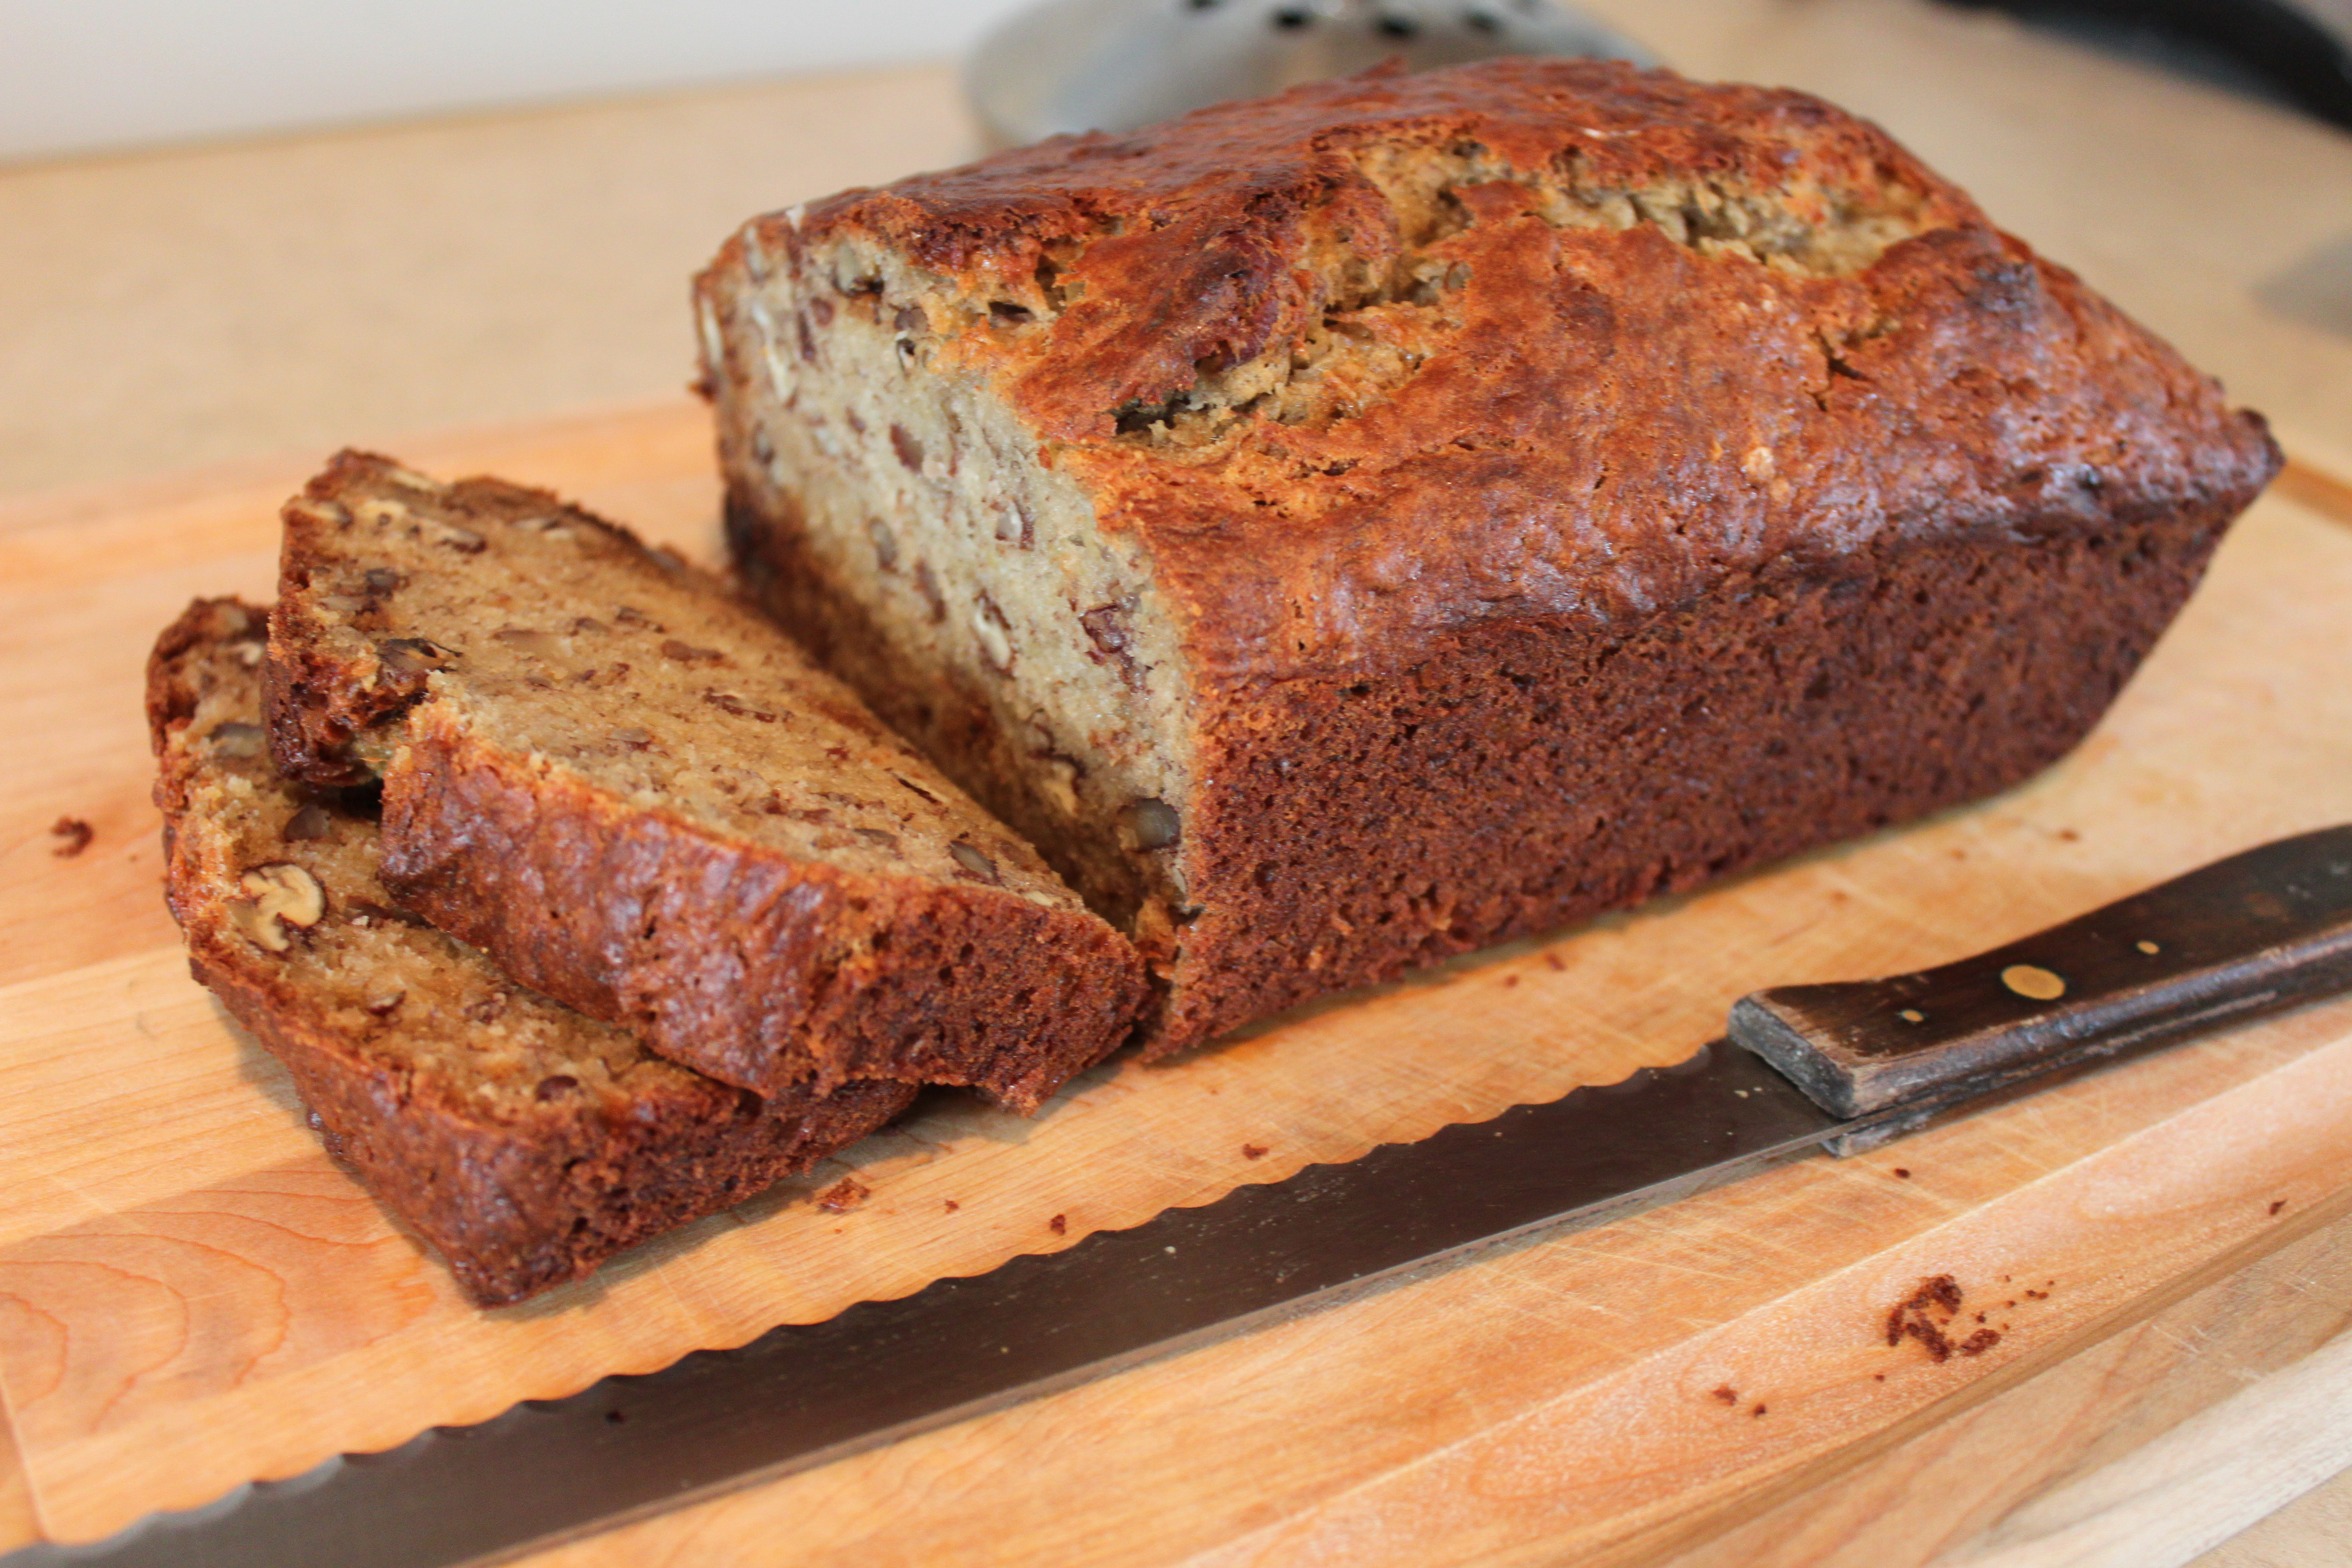
\includegraphics[height=0.26\textheight]{./figures/bananabread}
\end{center}
%\caption*{Yum.}
\end{figure}

%% \clearpage
\mysection{Thanksgiving}\label{thanksgiving}
%~~~~~~~~~~~~~~~~~~~~~~~~~~~~~~~~~~~~~~~~~~~~~~~~~~
%~~~~~~~~~ Turkey Figure ~~~~~~~~~~~~~~~~~~~~~~~~~~
%~~~~~~~~~~~~~~~~~~~~~~~~~~~~~~~~~~~~~~~~~~~~~~~~~~
%% \begin{figure}[h]
%% \begin{center}
%% 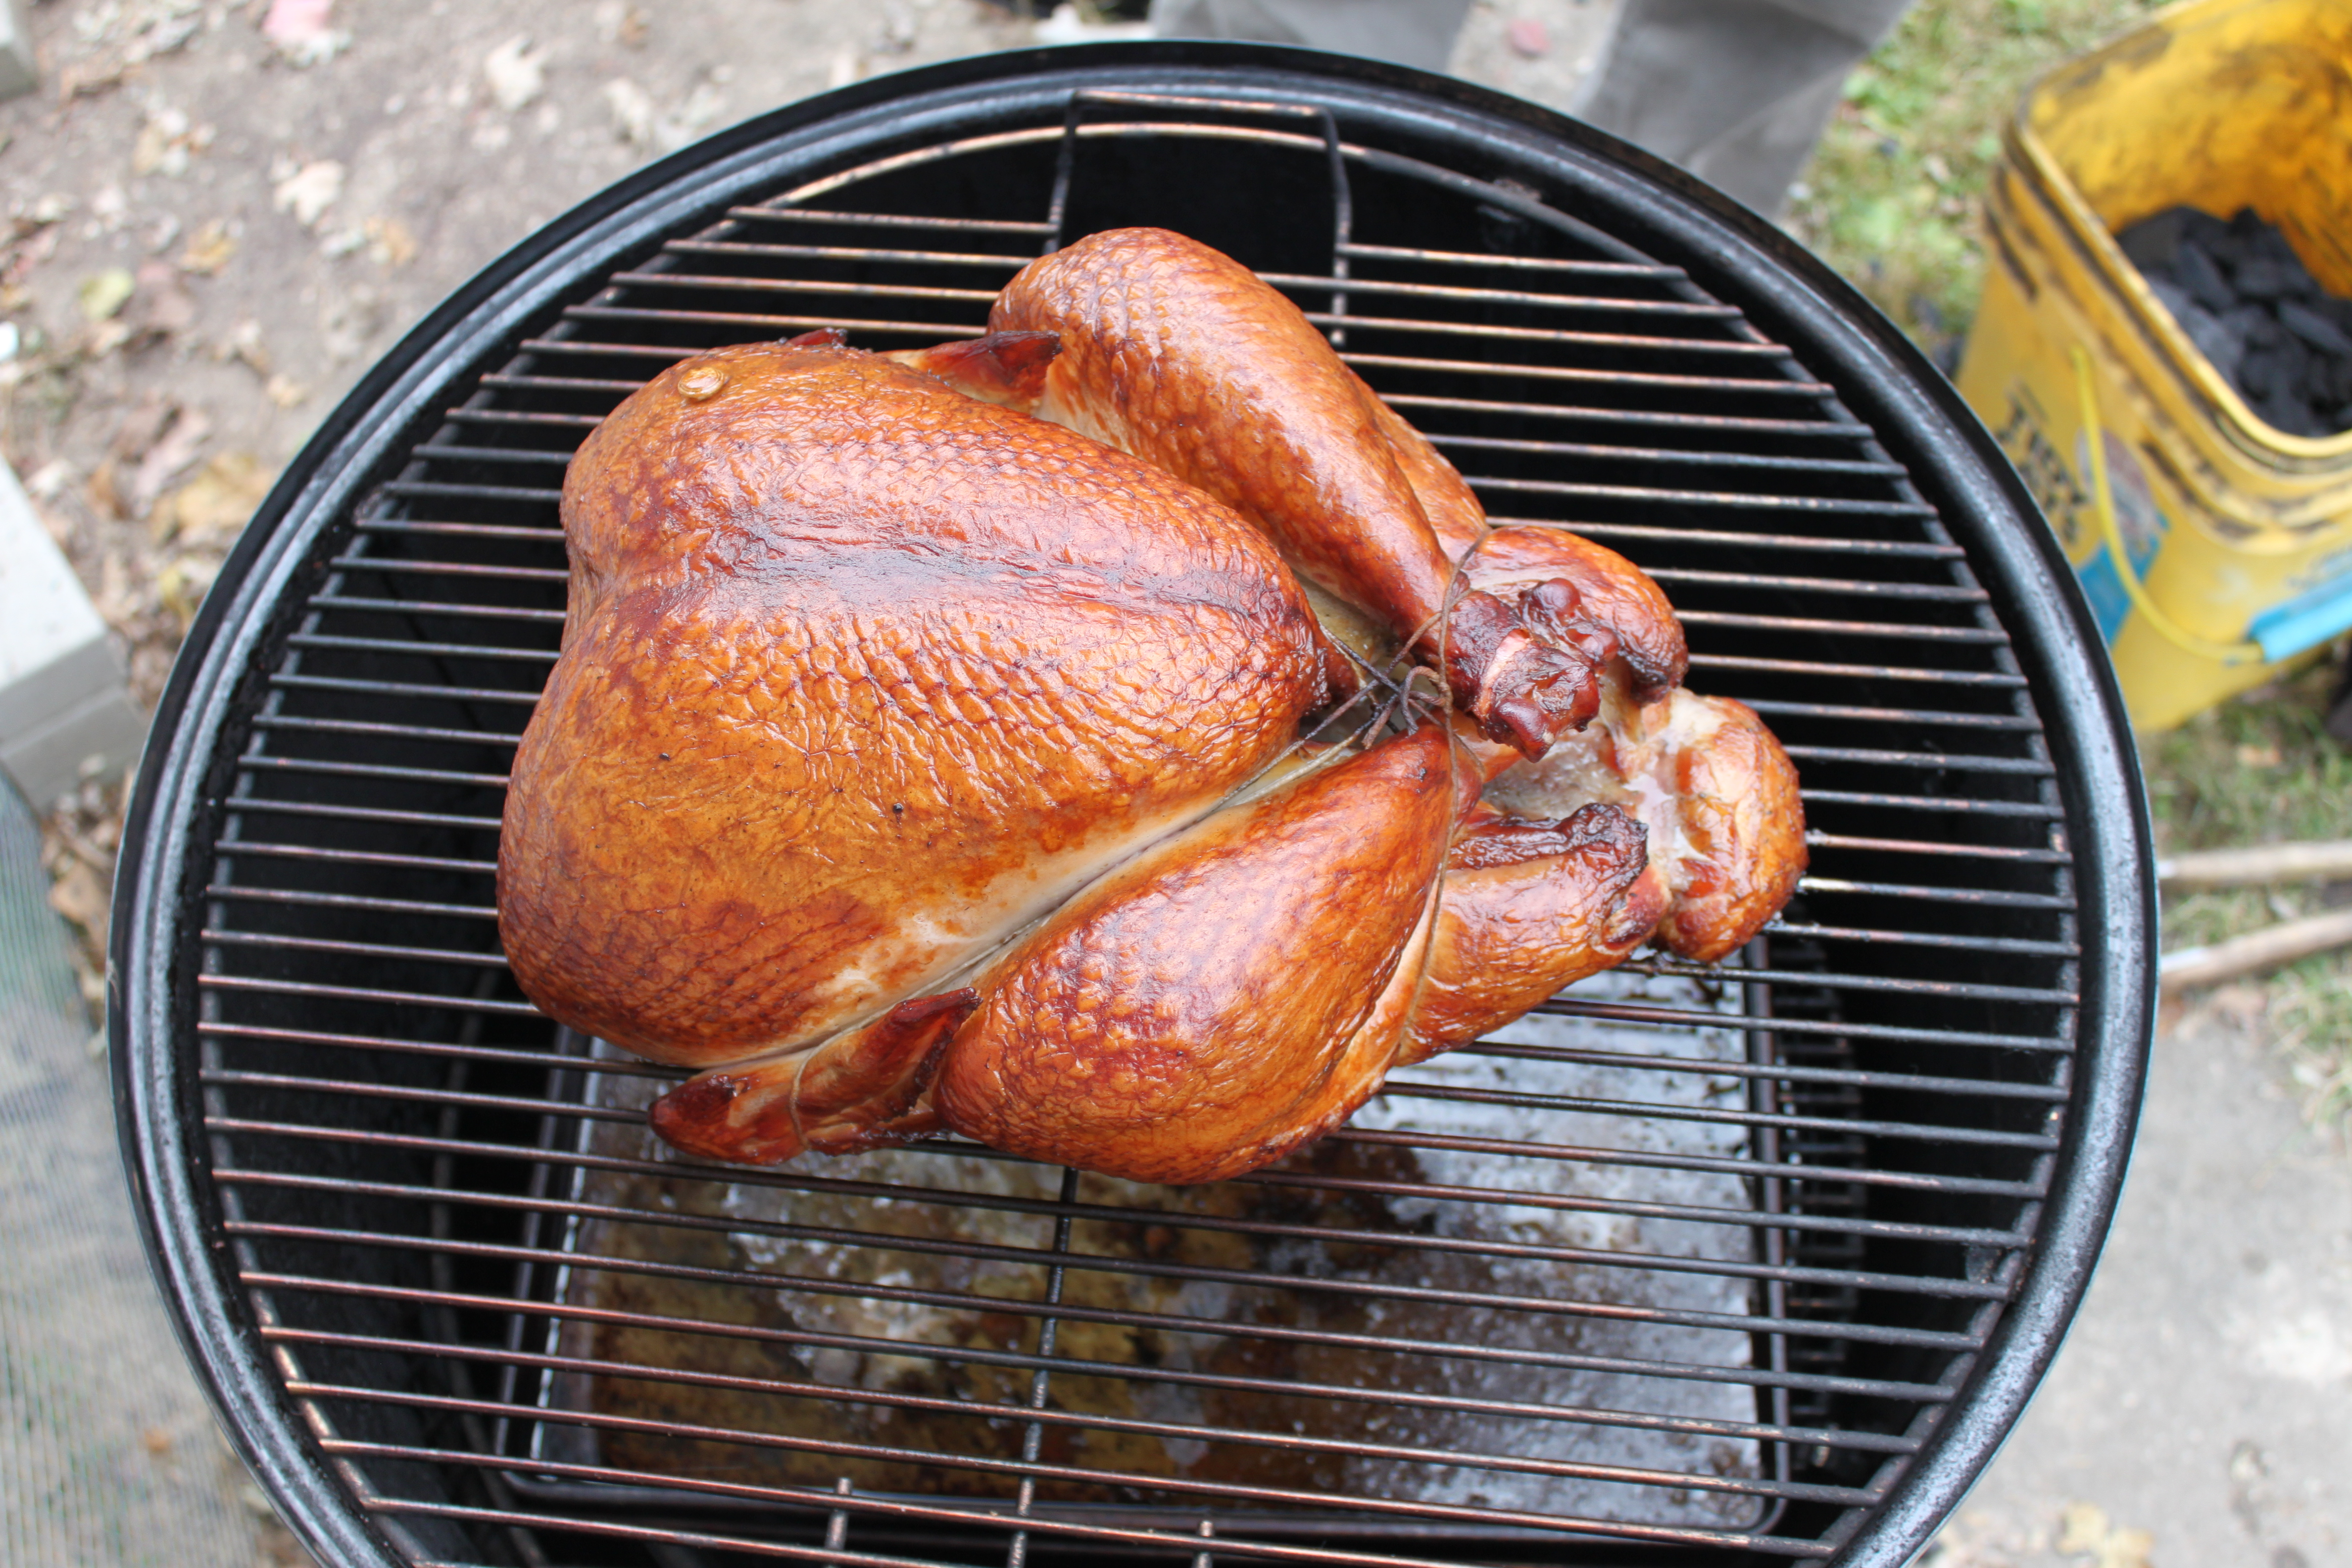
\includegraphics[width=0.6\textwidth]{./../figures/turkey}
%% \end{center}
%% \caption*{Turkey on the barbecue. Baltimore, 201?}
%% \end{figure}
%~~~~~~~~~~~~~~~~~~~~~~~~~~~~~~~~~~~~~~~~~~~~~~~~~~
%~~~~~~~~~~~~~~~~~~~~~~~~~~~~~~~~~~~~~~~~~~~~~~~~~~
%~~~~~~~~~~~~~~~~~~~~~~~~~~~~~~~~~~~~~~~~~~~~~~~~~~
\index{Sailor's Duff}
\begin{recipe}{Sailor's Duff}{8 servings}{1\fr14 hours}
\freeform This is a steamed molasses pudding served every year by the Buss family.  It requires a double-decker steamer and it is preferable to use un-sulfured molasses.
\ing[1]{c.}{dark molasses}
\ing[1]{c.}{cold water}
\ing[1]{}{egg}
Beat molasses, water and egg with mixer.
\ing[1\fr12]{c.}{flour, sifted}
Gradually sift in flour to molasses mixture.
\ing[1]{tsp}{\bs{}}
\ing[\fr12]{tsp}{salt}
Add \bs{} and salt to mixture.
\newstep
Pour mixture into greased \unit[8]{in.} spring-form pan or equivalent.  Steam in double-decker steamer on stove over boiling water for \unit[1]{hour}. Be sure to add enough water so that it does not boil dry.
\end{recipe}

\index{Sailor's Duff!Duff Sauce}
\begin{recipe}{Duff Sauce}{}{}
\freeform This is the sauce that accompanies Sailor's Duff.
\ing[1]{}{egg}
\ing[1]{c.}{granulated sugar}
\ing[1]{tsp.}{vanilla extract}
Combine egg, sugar and vanilla.  Let stand in a bowl for about an hour.  Just before serving whip cream and fold in egg mixture.
\ing[\fr12]{pint}{whipping cream}
\end{recipe}

\begin{recipe}{Dressing/Stuffing}{Serves 8}{1 hour}
\freeform From Laurie Stuart.
\newstep Preheat oven to \unit[350\0]{F.}
\ing[3]{}{onions, chopped}
\ing[1]{}{bunch of celery stalks, chopped}
\ing[12]{tbsp}{butter}
Saute\'{e} the onions and celery in the butter.
\newstep
Transfer onions, celery and butter to a large bowl.
\newstep
\ing[16]{oz.}{bag of croutons}
\ing[1]{batch}{corn bread}
Add croutons and crumble cornbread into celery and onions.
\newstep
\ing[16]{oz.}{chicken broth}
Moisten croutons and cornbread with chicken broth.
\newstep
\ing[]{}{salt \& pepper}
Season to taste.
\newstep
\ing[]{}{}
Transfer to an oiled oven-proof dish, and bake at \unit[350\0]{F.}, covered, for 30--45 minutes.
\end{recipe}

\begin{recipe}{Holiday Onion Casserole}{6 servings}{30 minutes}
\freeform This is the creamed onion dish Linda Younkin has served for holidays over the years.  It may be difficult to find pearl onions.\\
\newstep Preheat oven to \unit[400\0]{F.}
\ing[2]{tbsp}{butter}
\ing[2]{tbsp}{flour}
Melt butter and stir in flour.
\ing[\fr34]{c.}{milk}
\ing[1]{cube}{chicken bouillon}
Add milk and bouillon cube.  Cook, stirring often until mixture boils and thickens.
\ing[\fr12]{c.}{cheddar cheese, grated}
\ing[\fr12]{c.}{sherry}
Add cheese and sherry.  Stir over low heat until cheese melts.
\ing[]{}{salt \& pepper}
Season with salt \& pepper.
\ing[1]{lbs.}{pearl onions, canned or frozen}
Add onions.  Transfer to a greased casserole dish.
\ing[\fr14]{c.}{cheddar cheese, grated}
\ing[]{}{paprika}
Sprinke with more cheese and dust with paprika.
\newstep
Bake in an oven at 400\0 for about 20 minutes, or until bubbly and browned.
\end{recipe}

\index{Green Bean Casserole}
\begin{recipe}{Green Bean Mushroom Casserole}{Serves 6}{}
\freeform From Linda Younkin
\newstep Preheat oven to \unit[350\0]{F.}
\ing[10.5]{oz.}{canned cream of mushroom soup}
\ing[3]{tbsp.}{dry or medium sherry}
\ing[3]{c.}{drained cooked french style green beans}
\ing[1.75]{oz.}{canned french-fried onions}
Combine mushroom soup, sherry and green beans in a casserole dish.
\newstep Bake at \unit[350\0]{F.} for about \unit[25]{min.}
\ing[1.75]{oz.}{canned french-fried onions}
Crumble remaining onions over top, continue baking \unit[5]{min.}
\freeform ``I often omit the sherry, or put in only a little. I use frozen green beans, and cook them in the microwave.  I cook the beans in the microwave, drain them, add soup (and sherry), and half of the onions.'' Linda Younkin

\end{recipe}

\index{Bread!Cornbread}
\begin{recipe}{Corn Bread}{}{}
\freeform From Laurie Stuart.  Can be made a day in advance, and is useful for the dressing/stuffing recipe included here.
\newstep Preheat oven to 400\0.
\ing[1\fr12]{c.}{\apf{}}
\ing[\fr12]{c.}{corn meal}
\ing[\fr12]{c.}{sugar}
\ing[2]{tsp}{\bp{}}
\ing[\fr12]{tsp}{salt}
Combine dry ingredients.
\ing[1]{c.}{milk}
\ing[\fr12]{c.}{vegetable oil}
\ing[1]{}{egg, beaten}
Stir in wet ingredients, mixing just until dry ingredients are moistened.  Pour into greased pan and bake for 20--25 minutes, until light golden-brown.
\end{recipe}

\index{Soup!Turkey}
\begin{recipe}{Turkey Soup}{8 servings}{2\fr12 hours}
\freeform This  is Laurie Buss' classic post-Thanksgiving recipe. With leftover turkey, Linda Younkin also prepares a variation of this soup and Turkey Tetrazzini from the Joy of Cooking.
\ing[1]{}{turkey carcass}
\ing[~3]{qts}{chicken broth}
\ing[3]{}{carrots}
\ing[3-4]{stalks}{celery}
\ing[3]{}{bay leaves}
Place the turkey carcass, whole scrubbed carrots, whole rinsed celery stalks and bay leaves in a large pot. Add enough chicken broth to cover the carcass and boil for approximately \unit[45]{minutes} to an hour.
\newstep Remove the carcass and all bones. Strain the remaining solids from the broth and reserve. Pick all of the meat off of the carcass and bones and add back in to the broth.
\ing[3-4]{stalks}{celery}
\ing[28]{oz}{canned plum tomatoes}
Chop the fresh celery and roughly chop the drained tomatoes, adding both back in to the broth. Simmer for 30 minutes.
\ing{}{rice or egg noodles}
If you choose to use rice, add in a cup or a cup and a half at this step and simmer for 20 minutes then serve. If you choose to use noodles, add about two cups of egg noodles, simmering until tender. Season with salt and pepper to taste.
\freeform A turkey carcass should have a reasonable amount of meat remaining on it after the majority has been carved off. You can also chop up and add leftover meat from other pieces at step 2. If you have smoked your turkey, we find it best to remove the skin from the carcass before step 1.
\end{recipe}

\clearpage
\mysection{Sourdough Bread}\label{sourdough}
\index{Sourdough Bread!Sourdough Starter!Basic Feeding}
\begin{recipe}{Basic Feeding}{\unit[225]{g.}}{5 minutes}
\freeform A starter kept at room temperature should be fed once a day.\\
\rule{\textwidth}{0.05pt}
\hspace*{10mm}
\ing[50]{g.}{sourdough starter}
\ing[110]{g.}{water}
Whisk together. Use water that is at room temperature.
\ing[90]{g.}{rye flour}
Mix in flour thoroughly and transfer \unit[225]{g.} to a pint jar. Discard the rest.
\end{recipe}

\index{Sourdough Bread!Sourdough Starter!Large Feeding}
\begin{recipe}{Large Feeding}{\unit[225]{g.}, \unit[100]{g.}}{5 minutes}
\freeform Our sourdough bread recipe calls for \unit[185]{g.} of ripe starter. That doesn't leave much of the \unit[225]{g} from the basic feeding recipe leftover for continuing the starter. So we use this recipe prior to baking.\\
\rule{\textwidth}{0.05pt}
\hspace*{10mm}
\ing[65]{g.}{sourdough starter}
\ing[150]{g.}{water}
Whisk together. Use water that is at room temperature.
\ing[120]{g.}{rye flour}
Mix in flour thoroughly.
\freeform  Transfer \unit[225]{g.} to a pint jar and reserve \unit[100]{g.} to be fed the next day. The larger portion will be used after ripening for about \unit[3]{hrs.}
\end{recipe}

\clearpage
\mysection{Miscellaneous}
\index{Chili!Cincinnati}
\begin{recipe}{Cincinnati Chili}{6 servings}{3 hours}
\freeform Cincinnati chili recipe taken from ``Joy of Cooking.''\\
\rule{\textwidth}{0.05pt}
\ing[1]{qt.}{water}
Boil water in a \unit[4--6]{qt.} pot.
\ing[2]{lbs.}{ground chuck}
Add beef to boiling water and stir until separated.  Reduce heat and simmer.
\ing[2]{}{onions, medium}
\ing[5--6]{cloves}{garlic}
\ing[15]{oz.}{can of tomato sauce}
\ing[2]{tbsp.}{cider vinegar}
\ing[1]{tbsp.}{\ws{}}
Add to beef.
\ing[10]{}{peppercorns, ground}
\ing[8]{}{whole allspice, ground}
\ing[8]{}{whole cloves, ground}
\ing[1]{}{large bay leaf}
\ing[2]{tsp.}{salt}
\ing[2]{tsp.}{cinnamon, ground}
\ing[1\fr12]{tsp.}{cayenne pepper, ground}
\ing[1]{tsp.}{cumin, ground}
\ing[\fr12]{oz.}{unsweetened chocolate, grated}
Stir and add.
\end{recipe}

\index{Barbecue Baked Beans}
\begin{recipe}{Barbecue Baked Beans}{6 servings}{20 minutes}
\ing[1\fr12]{lbs.}{Italian sausage}
Brown in large saucepan and drain off fat.
\ing[1]{can}{baked beans}
\ing[1]{can}{Hormel\textsuperscript{\texttrademark} chili}
\ing[1]{can}{kidney beans}
\ing[1]{can}{vegetables, drained}
Add to sausage.
\ing[\fr12]{c.}{barbecue sauce}
\ing[1]{c.}{brown sugar}
Add ``secret ingredients'' and cook.
\end{recipe}

\index{Lobster!Grilled}
\begin{recipe}{Grilled Lobster}{}{}
\freeform Each year Linda sends us four lobsters for Sam's birthday on
March 2.  We usually boil two and grill two so that all four can be
cooked simultaneously and we can compare the merits of the two
grilling methods.  First we present the recipe for grilling.\\
\ing[2]{}{live lobsters}
Steam, covered, in two inches of water for 3\fr12 minutes to kill
the lobsters so you don't have to chop them in half while they are
still alive.  Remove and let cool until they can be handled, ten to
fifteen minutes.\\
\freeform Cut the lobsters in half straight down the middle from
between the eyes through the tail.  Do not remove any of the yucky
stuff.  Place the four lobster halves shell side down on a hot grill.  Heat is
good, but singed shell is bitter, so avoid a large flame.\\
\ing[4]{tbsp}{butter, melted}
After the lobsters have been on the grill for about five minutes brush
with melted butter.  Cover the grill and cook for another five minutes
or so.\\
\freeform We have found that grilled tails are great, but the claws
are better boiled.  It is also quite awkward to cook both the tail and
claw when on the grill.  Next time we will try grilling the tails
and boiling the claws.
\end{recipe}

%%\rule{\textwidth}{0.05pt}
%\newstep Wait fo two weeks.  Skim periodically.
%\ing[\fr12]{c.}{salt}

\index{Chili!Powder}
\begin{recipe}{Chili Powder}{about \unit[1]{cup}}{1 hour}
\ing[55]{gr.}{guajillo chiles, dried\\(\unit[2.5--5]{kSc.})}
\ing[14]{gr.}{coste\~{n}o chiles, dried\\(\unit[7--10]{kSc.})}
\ing[10]{gr.}{datil chiles, dried\\(\unit[100--300]{kSc.})}
Stem, slice and seed chiles. Weigh the chiles after stemming and seeding.  Wear latex gloves.
\ing[20]{gr.}{whole cumin seed}
Toast the chiles with the cumin for about \unit[3--4]{minutes} moving constantly on a dry skillet.  Let chile and cumin cool.
\ing[1]{tsp}{garlic powder}
\ing[4]{tsp}{dried oregano}
\ing[1]{tsp}{paprika}
Grind chiles and cumin along with other spices until a fine powder.
\end{recipe}

\index{Red Pepper Relish}
\begin{recipe}{Sweet Red Pepper Relish}{}{}
\rule{\textwidth}{0.05pt}
\ing[12]{}{large green bell peppers}
\ing[12]{}{red bell peppers}
\ing[3]{}{small hot peppers}
\ing[6]{}{large onions}
Chop vegetables, finely, or use a food processor.
\ing[\fr12]{c.}{salt, non-iodized}
Transfer chopped vegetables to a bowl and mix with salt.
\ing[\fr12]{gal.}{boiling water}
Pour hot water over mixture and let stand for \unit[15]{minutes}.
\newstep Drain well.
\ing[2]{tsp.}{celery seed}
\ing[2\fr12]{c.}{sugar}
Mix in  celery seed and sugar.
\ing[2]{c.}{cider vinegar}
Cover mixture with cider vinegar.
\newstep Put in \emph{strike jars}\ldots
\end{recipe}

\index{Peanuts!Honey roasted}
\begin{recipe}{Honey Roasted Peanuts}{\unit[1]{pound}}{\unit[40]{minutes}}
\freeform Sam makes honey roasted peanuts around Christmas time. Packaged nicely in a jar or tin, they make and excellent gift and keep well in an air-tight container.
\newstep Preheat oven to \unit[325\0]{F.} Line a baking sheet with aluminum foil and spray with cooking spray. 
\ing[2]{tbsp}{butter}
\ing[\fr13]{c.}{honey}
\ing[1]{tsp}{vanilla extract}
Melt the butter, honey and vanilla together over low heat, stirring until smooth.
\ing[1]{lb}{Shelled Virginia peanuts}
Stir peanuts and honey mixture together and spread out on prepared baking sheet. Bake 20 minutes, stirring every 5 minutes to ensure even baking. Be sure to stir up edges of the pan as they tend to burn. When golden brown, remove from the oven and stir once more.
\ing[\fr14]{c.}{sugar}
\ing[1]{pinch}{granulated salt, to taste depending on the saltiness of peanuts used}
Two minutes after removing from the oven, sprinkle peanuts with the sugar and pinch of salt. Be sure to allow nuts to cool completely before removing from the sheet pan to eat, store or package.
\end{recipe}
%% \begin{figure}[b!]
%% \begin{center}
%% \includegraphics[height=0.25\textwidth]{./../figures/chemex}
%% \hspace{0.1\textwidth}
%% \includegraphics[height=0.25\textwidth]{./../figures/chemex-2}
%% \hspace{0.1\textwidth}
%% \end{center}
%% \caption*{The Chemex Coffee Maker}
%% \end{figure}
\index{Coffee!Chemex}
\begin{recipe}{Chemex\textsuperscript{\texttrademark} Coffee Maker}{3 servings}{10 minutes}
\ing[?]{c.}{water, boiled}
Place filter in Chemex\textsuperscript{\texttrademark} coffee maker.  Pour about half of a cup of hot water (around \unit[200\0]{F}) through the filter, and dump water in sink.  The point of this is to warm and clean the filter, and make it adhere more readily to the glass.
\ing[?]{c.}{coffee, coarsely ground}
Add coffee grounds to filter.  Pour about half of a cup of hot water gently over the grounds.  Watch the grounds ``bloom,'' during which, if the beans are fresh, the coffee grounds will expand and bubble.  Only use enough water to moisten the grounds.
\newstep
Slowly fill Chemex\textsuperscript{\texttrademark} coffee maker with hot water (around \unit[200\0]{F}) and let strain.  When finished straining, refill with hot water, and strain again.  It may be necessary to reheat the water for second batch of straining.
\newstep
Transfer coffee to carafe or thermos.
\end{recipe}
\begin{figure}[b!]
\begin{center}
\includegraphics[height=0.25\textwidth]{\string~/Dropbox/cookbook/figures/chemex}
\hspace{0.1\textwidth}
\includegraphics[height=0.25\textwidth]{\string~/Dropbox/cookbook/figures/chemex-2}
\end{center}
\caption*{The Chemex\tm{} Coffee Maker}
\end{figure}

%\clearpage
\mychapter{Denver}
\mysection{Small Dish}\label{smalldishes}
\index{Dumplings!Shu Mai}
\begin{recipe}{Shrimp and Cilantro Shu Mai}{Yield 10 to 12 dumplings}{30 minutes}
\freeform Not sure where we found this recipe, but we've had fun with it, especially for make-your-own dumpling kids' birthday parties. If you've got some bamboo steamers, you can do multiple levels at once. Parchment steamer liners keep dumplings from sticking. A steaming ring lets you place everything over a stock pot.\\
\rule{\textwidth}{0.05pt}

\ing[\fr12]{c}{soy sauce}
\ing[1]{tbsp}{rice wine}
\ing[1]{tbsp}{sesame oil}
\ing[1]{tbsp}{minced fresh ginger}
Combine the soy sauce, rice wine, sesame oil, and ginger in a bowl.

\ing[\fr12]{pound}{shrimp, peeled and deveined}
\ing[\fr34]{c}{cilantro leaves}
\ing[\fr14]{c}{roughly chopped scallions, white parts only}
Put half the shrimp, half the cilantro, and all the scallions in a food processor and pulse; add just enough of the soy mixture to create a smooth paste, about 1 to 2 tablespoons. Transfer to a bowl. Roughly chop the remaining shrimp and cilantro, add them to the bowl and stir to combine.

\ing[10 to 12]{}{round dumpling skins}
Place a dumpling skin on a work surface, moisten the edges with water, and put 1 teaspoon of the filling in the center. Gather the edges of the wrapper up around the filling, squeezing gently, to pleat the sides; some of the filling should remain exposed. Repeat with the remaining dumpling skins and filling, keeping the dumpling wrappers and dumplings covered with damp towels while you work.

\ing[]{}{juice of 1 lime}
Rig a steamer in a large pot over an inch of water; bring to a boil and reduce to a simmer. Meanwhile, add the lime juice to the remaining soy mixture to make a dipping sauce.

\newstep
Put as many dumplings in the steamer as you can fit in a single layer and cover the pot. Cook until the exposed filling turns pink and the wrappers are tender, 4 to 6 minutes, then transfter the dumplings to a serving platter. Repeat with the remaining dumplings. Serve with the dipping sauce.

\end{recipe}
\mysection{Breakfast}
\index{Pancakes!World's Best}
\begin{recipe}{The World's Best Pancake Recipe}{}{}
\freeform This recipe is from Robie's Country Store in Hooksett,
NH. But it came to us through the ever watchful Jason
Kottke\\
\rule{\textwidth}{0.05pt}
\ing[2]{c.}{flour}
\ing[2]{tbsp}{sugar}
\ing[4]{tsp}{baking powder}
\ing[1]{tsp}{fine salt}
Combine the dry ingredients in a bowl, whisk, set aside:
\ing[2]{c.}{buttermilk}
\ing[4]{tbsp}{melted butter}
\ing[1]{tsp}{vanilla extract}
\ing[2]{}{beaten eggs}
Combine the wet ingredients in a second bowl, whisk:
\newline
\\
Add the wet ingredients to the dry and whisk until just combined. Fry
in a pan with butter. Top with maple syrup and devour.
\end{recipe}

\clearpage
\mysection{Main Dish}
\index{Chicken!Adobo}
\begin{recipe}{Chicken Adobo}{Serves Four}{}
\freeform The national dish of the Philippines. Adapted from Purple Yam Restaurant in Brooklyn by Sam Sifton of the NYTimes. We like to serve it over brown rice.\\
\rule{\textwidth}{0.05pt}

\ing[1\fr12]{c}{rice vinegar}
\ing[1]{c}{coconut milk}
\ing[\fr14]{c}{soy sauce}
\ing[12]{cloves}{peeled garlic}
\ing[1-2]{}{Thai hot peppers or a jalapeno, halved and seeded}
\ing[3]{}{bay leaves}
\ing[1\fr12]{tsp}{freshly ground black pepper}
\ing[3-4]{lbs}{chicken thighs}

Combine all of the marinade ingredients in a large, nonreactive bowl
or resealable plastic freezer bag. Add the chicken and turn to
coat. Refrigerate overnight or for at least 2 hours.

\freeform Place chicken and marinade in a large lidded pot or Dutch
oven over high heat and bring to a boil. Immediately reduce heat to a
simmer and cook, stirring occasionally, until the chicken is cooked
through and tender, around 30 minutes.  Heat broiler. Transfer chicken
pieces to a large bowl, raise heat under the pot to medium-high, and
reduce the sauce until it achieves almost the consistency of cream,
about 10 minutes. Remove bay leaves and hot peppers.  Place chicken pieces
on a roasting pan and place under broiler for 5 to 7 minutes, until
they begin to caramelize. Remove, turn chicken, baste with sauce and
repeat, 3 to 5 minutes more. Return chicken to sauce and cook for a
few minutes more, then place on a platter and drizzle heavily with
sauce.
\end{recipe}

\index{Stews!Garbanzos and Spinach}
\begin{recipe}{Garbanzos con Espinacas}{Serves 2 - 3}{1\fr12 hours}
\freeform
Spanish Chickpea and Spinach Stew with Ginger. From Serious Eats. This recipe happens to be vegan, but we don't hold that against it. Serve over brown rice.\\
\rule{\textwidth}{0.05pt}

\ing[1]{28 oz can}{ whole peeled tomatoes}
\ing[1]{1 inch knob}{ginger, peeled}

Drain tomatoes in a metal strainer set over a medium bowl. Transfer liquid and half of tomatoes to a blender along with ginger. Blend on high speed until completely pureed. Set aside. Roughly chop remaining peeled tomatoes and set aside separately.
\newline
\ing[\fr14]{cup}{extra-virgin olive oil}
\ing[1]{}{medium onion, finely sliced}
\ing[4]{cloves}{garlic, finely sliced}
\ing[1]{tsp}{sweet or hot smoked paprika}
\ing[12]{ounces}{fresh spinach, roughly chopped}

Heat olive oil in a large straight-sided skillet over high heat until shimmering. Add onion, garlic, and paprika, and cook, stirring frequently, until softened and very slightly browned. Add tomato-ginger puree (it should immediately start simmering) and stir to combine. Add spinach a handful at a time, allowing each handful to wilt before adding the next. Reduce heat to medium and allow spinach mixture to simmer, stirring occasionally, until spinach is completely tender, about 10 minutes.
\newline
\ing[2]{cans}{chickpeas}
\ing[2]{}{bay leaves}
\ing[2]{tsp}{soy sauce}

Add chopped tomatoes, garbanzo beans (with their liquid) bay leaves, and soy sauce, and bring to a boil over high heat. Reduce to a bare simmer and cook, stirring occasionally, until thickened into a thick stew, about 30 minutes total.
\newline
\ing[]{}{kosher salt}
\ing[]{}{sherry vinegar for serving (optional)}

Season to taste with kosher salt and serve immediately, drizzling with extra virgin olive oil and a a few drops of sherry vinegar.

\end{recipe}

\index{Flank Steak}
\begin{recipe}{Flank Steak}{}{}
\freeform A simple marinade for Flank Steak. Pairs nicely with white rice.\\
\rule{\textwidth}{0.05pt}

\ing[\fr13]{c}{lemon juice}
\ing[\fr13]{c}{canola oil}
\ing[\fr14]{c}{soy sauce}
\ing[2]{tbsp}{onion powder}
Combine all of the marinade ingredients in a gallon freezer bag.

\ing[1]{}{flank steak}
Add the steak and turn to coat. Refrigerate overnight, turning occasionally. Grill to medium-rare, rest 10 minutes, then slice thinly across the grain. 

\end{recipe}

\clearpage
\mysection{Dessert}
\index{Cookies!Chocolate Chip!Spiced Oatmeal}
\begin{recipe}{Spiced Oatmeal Chocolate Chip Cookies}{Yield 20 to 24 Cookies}{}
\freeform
From the Chocolate Bar Cookbook. Sarah and I reduced the sugar by 1/3
after hearing an inspirational NPR interview. I swear they taster
better this way - perhaps more savory. Oh, and we sprinkle them with
sea salt. Maldon's if you want to get real fancy.\\
\rule{\textwidth}{0.05pt}
\ing[1\fr34]{c}{unbleached flour}
\ing[1]{tsp}{baking soda}
\ing[1]{tsp}{salt}
\ing[1]{tsp}{ground cinnamon}
Sift the flour, baking soda, salt and cinnamon together and set aside.
\ing[2]{sticks}{unsalted butter, softened}
\ing[\fr34]{c}{dark brown sugar}
\ing[\fr16]{c}{granulated sugar}
In a medium size mixing bowl, cream the butter with both sugars until
smooth.
\ing[2]{}{eggs}
\ing[2]{tsp}{vanilla extract}
Add the eggs and vanilla, beating until very fluffy. You may use an
electric mixer if desired.
\ing[2\fr34]{c}{whole oats}
\ing[12]{oz}{bittersweet chocolate pieces, or chopped chunk chocolate}
\ing[]{}{sea salt flakes}
Add the sifted ingredients, mixing thoroughly until the batter is
smooth. Add the oats and chocolate, mixing until just blended. Chill
the dough for at least 6 hours.
\freeform
Preheat the oven to 350 degrees. Drop by tablespoonfuls, about 1\fr12
each, on an ungreased baking sheet. Sprinkle with sea salt
flakes. Bake for 13 to 15 minutes. Once finished baking, allow the
cookies to cool for 8 to 10 minutes before transferring to a cooling
rack.
\end{recipe}
\index{Pie!Lemon Meringue}
\begin{recipe}{Lemon Meringue Pie}{}{}
\freeform
This recipe, better known in our house as LMNOP, is a Margie Goldberg
classic. Originally from the James Beard Cookbook, it's a bit of a
challenge, but well worthwhile.\\
\rule{\textwidth}{0.05pt}

\ing[1]{large}{egg yolk}
\ing[2]{tbsp}{ice water}
\ing[1]{tbsp}{lemon juice}
\ing[1]{pinch}{salt}
\ing[1]{stick}{butter}
\ing[1\fr12]{c}{AP flour}
\ing[2]{tbsp}{sugar}

\textbf{The Pastry}\\
Beat yolk lightly and add ice water, lemon juice, and salt. Cut or
work butter into flour, then add, along with sugar, to the egg
mixture. Work ingredients together until they form a soft ball. Chill
for \fr12 hour and pat into a flan ring or 9-inch tin. Place a piece
of foil inside shell and fill with pie weights. Bake at 350 for 25 to
30 minutes. Remove weights.


\ing[6]{}{egg yolks}
\ing[1\fr12]{c}{sugar}
\ing[1]{}{grated lemon rind}
\ing[\fr12]{c}{lemon juice}
\ing[3]{tbsp}{butter}
\ing[4]{tbsp}{cornstarch}
\ing[\fr14]{tsp}{salt}
\ing[1\fr12]{c}{boiling water}

\textbf{The Filling}\\
Beat egg yolks well, add remaining ingredients except boiling water,
and beat again thoroughly. Combine with boiling water and pour into
top of double boiler. Cook over hot water till mixture thickens, and
allow to cook for 5 to 10 minutes longer over simmering water. Pour
into baked shell. Top with meringue.

\ing[3]{}{egg whites}
\ing[1]{tsp}{cream of tartar}
\ing[1]{pinch}{salt}
\ing[6]{tbsp}{sugar}

\textbf{The Meringue}\\
Beat egg whites till they form soft peaks. Add cream of tartar and
salt and continue beating till whites are stiff but not dry. Add
sugar, a little at a time, beating it in well. Spread meringue over
the pie, being certain to cover the surface completely, including the
edge of the crust. If you are deft with the pastry tube, you may pipe
the meringue over the pie, using a number 6 rosette tube. Bake the
meringue at 350 for 15 to 18 minutes, or until it is lightly browned.

\end{recipe}

%\clearpage
\mychapter{Ponte Vedra Beach}
\mysection{Main Dish}\label{pvb}
\index{Jambalaya!Roast Chicken}
\index{Stew!Jambalaya!Roast Chicken}
\begin{recipe}{Roast Chicken Jambalaya}
{\unit[6]{servings}}{\unit[45]{minutes}}
\freeform This recipe from Steve Younkin was adapted from one pulled
from the internet. The sausage makes this dish so find a sausage you
like in your jambalaya. Steve always uses Savoie andouille, and avoids
other brands. You can add almost any meat to jambalaya (e.g. shrimp
which will cook well if you add them raw after the rice is done, or
white meat chicken).
\ing[5]{oz}{Andouille sausage}
\ing[2-3]{tbsp}{olive oil}
Slice the sausage into quarter inch slices, then pile up 3 slices and
cut the stack into quarters. Repeat until all the sausage is in
quarter inch pieces. Add the sausage to olive oil in an enameled cast
iron pot over medium heat. Make sure the flat surface of each piece of
sausage is down on the pan. I prefer Savoie Andouille sausage.
\ing[1]{large}{white onion}
While the sausage is cooking, dice the onion into quarter inch pieces
and layer gently over the sausage so that the sausage continues to
brown.
\ing[5-8]{stalks}{celery}
Next dice the celery into quarter inch pieces, add to the pot, and mix
everything up getting any brown bits off the bottom of the pan.
\ing[1]{}{red pepper}
Next dice the red pepper into quarter inch pieces and add to the pot.
\ing[1]{tsp}{dried thyme}
\ing[1]{tsp}{dried oregano}
\ing[1-2]{tbsp}{dried basil}
Next add the basil, thyme, and oregano. Mix well and cook for 3-5
minutes to wilt the vegetables completely and release the oil from the
herbs.
\ing[2]{cups}{vegetable or chicken stock}
\ing[1]{cup}{white rice}
Add stock (I prefer Kitchen Basics) and white rice. Bring to a boil
and sprinkle salt lightly over the entire surface of the stock. Reduce
the heat to very low, cover and allow the rice to absorb the flavorful
stock for 15 minutes.
\ing{}{chicken, dark meat, roasted}
Cut the dark meat from an entire roasted chicken into bite
sized pieces and mix into the rice.\\
\freeform Test to make sure the rice is completely done (cook longer if
needed) then let the jambalaya sit for 5-10 minutes to completely warm
up the chicken. Serve with warm bread.
\end{recipe}

\clearpage
\printindex
\end{document}
%% %\newpage
%% \begin{recipe}{Sauerkraut}{}{}
\freeform Sauerkraut.
%%\rule{\textwidth}{0.05pt}
\ing[\fr12]{c.}{cabbage, shredded or finely chopped.}
\ing[\fr12]{c.}{salt}
Combine in crock.
\newstep Wait fo two weeks.  Skim periodically.
\end{recipe}

%%\newpage
%\mysection{The Less Favorites}\label{lessfavorites}
%\begin{recipe}{Basic Rib Rub}{about 1\fr12 cups}{15 minutes}
\freeform Taken from \emph{\path{allrecipes.com}}. We used this recipe with Sam's Chili powder \#4, recipe number \string~/\ref{sam4} to make pork spare ribs in the smoker.  May 1, 2011.
\ing[\fr12]{cup}{packed brown sugar}
\ing[2]{tbsp}{chili powder}
\ing[1]{tbsp}{paprika}
\ing[1]{tbsp}{freshly ground black pepper}
\ing[2]{tbsp}{garlic powder}
\ing[2]{tsp}{onion powder}
\ing[2]{tsp}{kosher salt}
\ing[2]{tsp}{ground cumin}
\ing[1]{tsp}{ground cinnamon}
\ing[1]{tsp}{~o seasoning salt (optional)}
Combine all ings and store in an air-tight container.
%\freeform\hrulefill
\end{recipe}

%%\newpage
%
\begin{recipe}{Basic Barbecue Mop}{about 2 cups}{15 minutes}
\freeform Taken from \emph{\path{allrecipes.com}}.
\ing[1]{cup}{apple cider}
\ing[\fr34]{cup}{apple cider vinegar}
\ing[1]{tbsp}{onion powder}
\ing[1]{tbsp}{garlic powder}
\ing[2]{tbsp}{lemon juice}
\ing[1]{}{~o pepper, finely chopped (optional)}
\ing[3]{tbsp}{hot pepper sauce}
\ing{}{kosher salt}
\ing{}{black pepper}
Combine all ingredients and mix.
\freeform We didn't use hot sauce, but we did use the ~o.  We used this mop on pork spare ribs rubbed with the basic rib rub \ref{}.  It was fine -- nothing to get too excited about.  Similar to what we normally used, and is thus the basic rib rub.
\end{recipe}

%\begin{recipe}{Lobster Stock}{3 qts}{2 hours}
\ing[4]{}{lobster carcasses}
Remove gills (and sand sac?) as well as any singed shell.
\ing[2]{}{onions, chopped}
\ing[6]{}{carrots, chopped}
\ing[4]{tbsp}{olive oil}
Sautee in a large stock pot until tender.
\ing[4]{cloves}{garlic, chopped}
\ing[6]{}{plum tomatoes, canned}
Add garlic and shells to stock pot and cook for a few minutes
\ing[1]{c.}{white wine}
Add white wine and cook off the alcohol.
\ing[4]{}{bay leaves}
\ing[]{}{black pepper, ground}
Add herbs and spices. Here we use bay leaves and black pepper, but
parsley is called for.
\ing[]{}{water} Add enough water to cover the shells by a few inches. Bring to a boil, and simmer for 60-90 minutes.\\
\freeform I also added some of the cooking water from the lobster boil.  Remove shells and pour stock through a medium filter or cheese cloth.  Return stock to the stove.\\
\ing[]{}{thyme}
\ing[]{}{red pepper flakes}
\ing[]{}{oregano}
Simmer the stock and season to taste.\\
\freeform The stock can be frozen in an ice cube tray and stored.
\end{recipe}

%%\rule{\textwidth}{0.05pt}
%\newstep Wait fo two weeks.  Skim periodically.
%\ing[\fr12]{c.}{salt}
%% \freeform

%%\newpage
%\begin{recipe}{Ginger Soy Sauce}{4 servings}{\unit[5]{min.}}
\freeform Great served on meat, fish or vegetables.
\ing[\fr12]{cup}{soy sauce}
\ing[\fr12]{cup}{balsamic vinegar}
\ing[1]{tsp}{crushed ginger or fresh grated ginger}
\ing[2]{tbsp}{water}
\ing[3--4]{tbsp}{chopped scallions}
\ing[\fr34]{tsp}{sugar}
\freeform Whisk all ings together until sugar is dissolved.
\end{recipe}

%%\newpage
%\begin{recipe}{Refried Beans}{\unit[4]{cups}}{\unit[3]{hours}}
\freeform Refried bean recipe taken initially from simplyrecipes.com.
\ing[2\fr12]{c.}{dried pinto beans}
\ing[1]{gallon}{water}
Rinse beans and discard any unpleasantries.  Cover beans with 4 inches
of water and boil.  Cover and simmer for \unit[2\fr12]{hours}.
\ing[2]{tbsp.}{butter}
\ing[1]{tbsp.}{olive oil}
\ing[\fr12]{}{onion, chopped}
Add butter and oil to large skillet and cook onions until translucent.
\newstep Strain beans and combine with onions in skillet.  Mash with a potato masher.
\ing[2]{tbsp.}{butter}
\ing[\fr12]{c.}{water}
Thin with water and butter to desired consistincy.
\ing[]{}{salt to taste}  Suggested seasonings; datil powder
\end{recipe}

%%\newpage
%~~~~~~~~~~~~~~~~~~~~~~~~~~~~~~~~~~~~~~
%% \begin{figure}
%% \begin{center}
%% \includegraphics[height=0.5\textwidth]{./../figures/datil-bite-me}
%% \end{center}
%% \caption*{Datil chili peppers on the plant at Joe's ``Bite Me Farms'' in St.\ Augustine, FL.}
%% \end{figure}
%% \begin{figure}
%% \begin{center}
%% 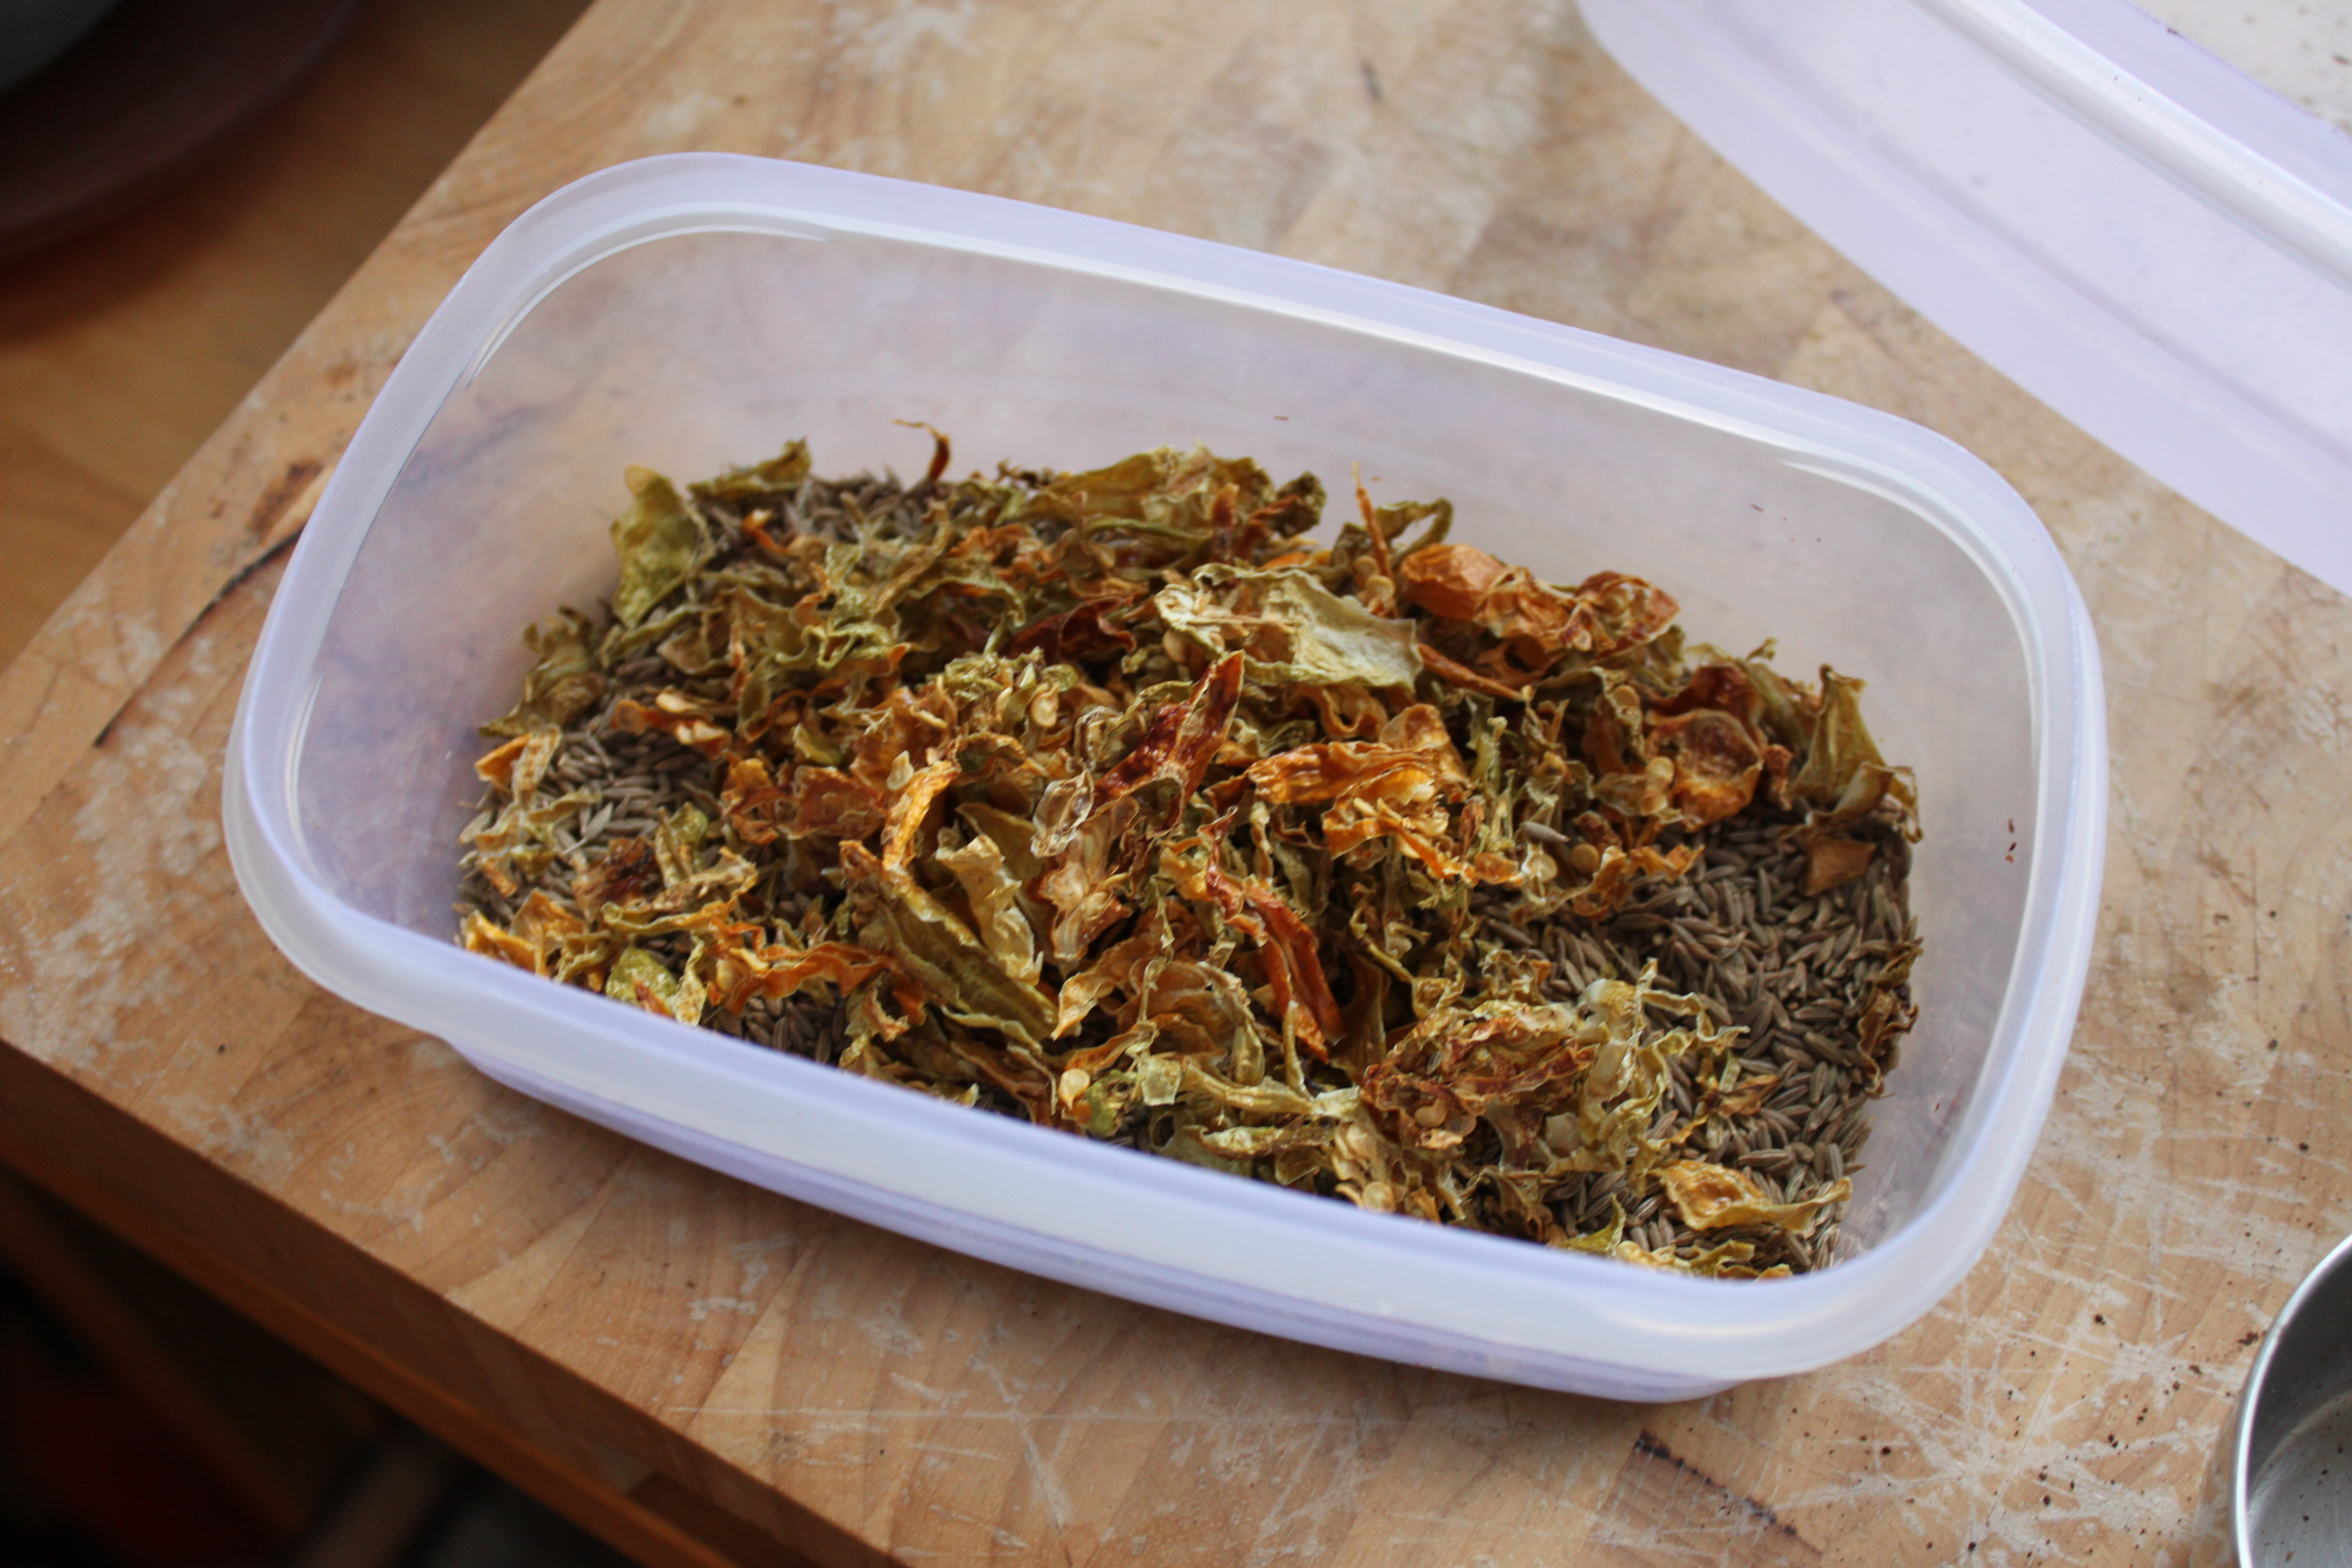
\includegraphics[height=0.3\textwidth]{./../figures/datil-sgy-2}
%% 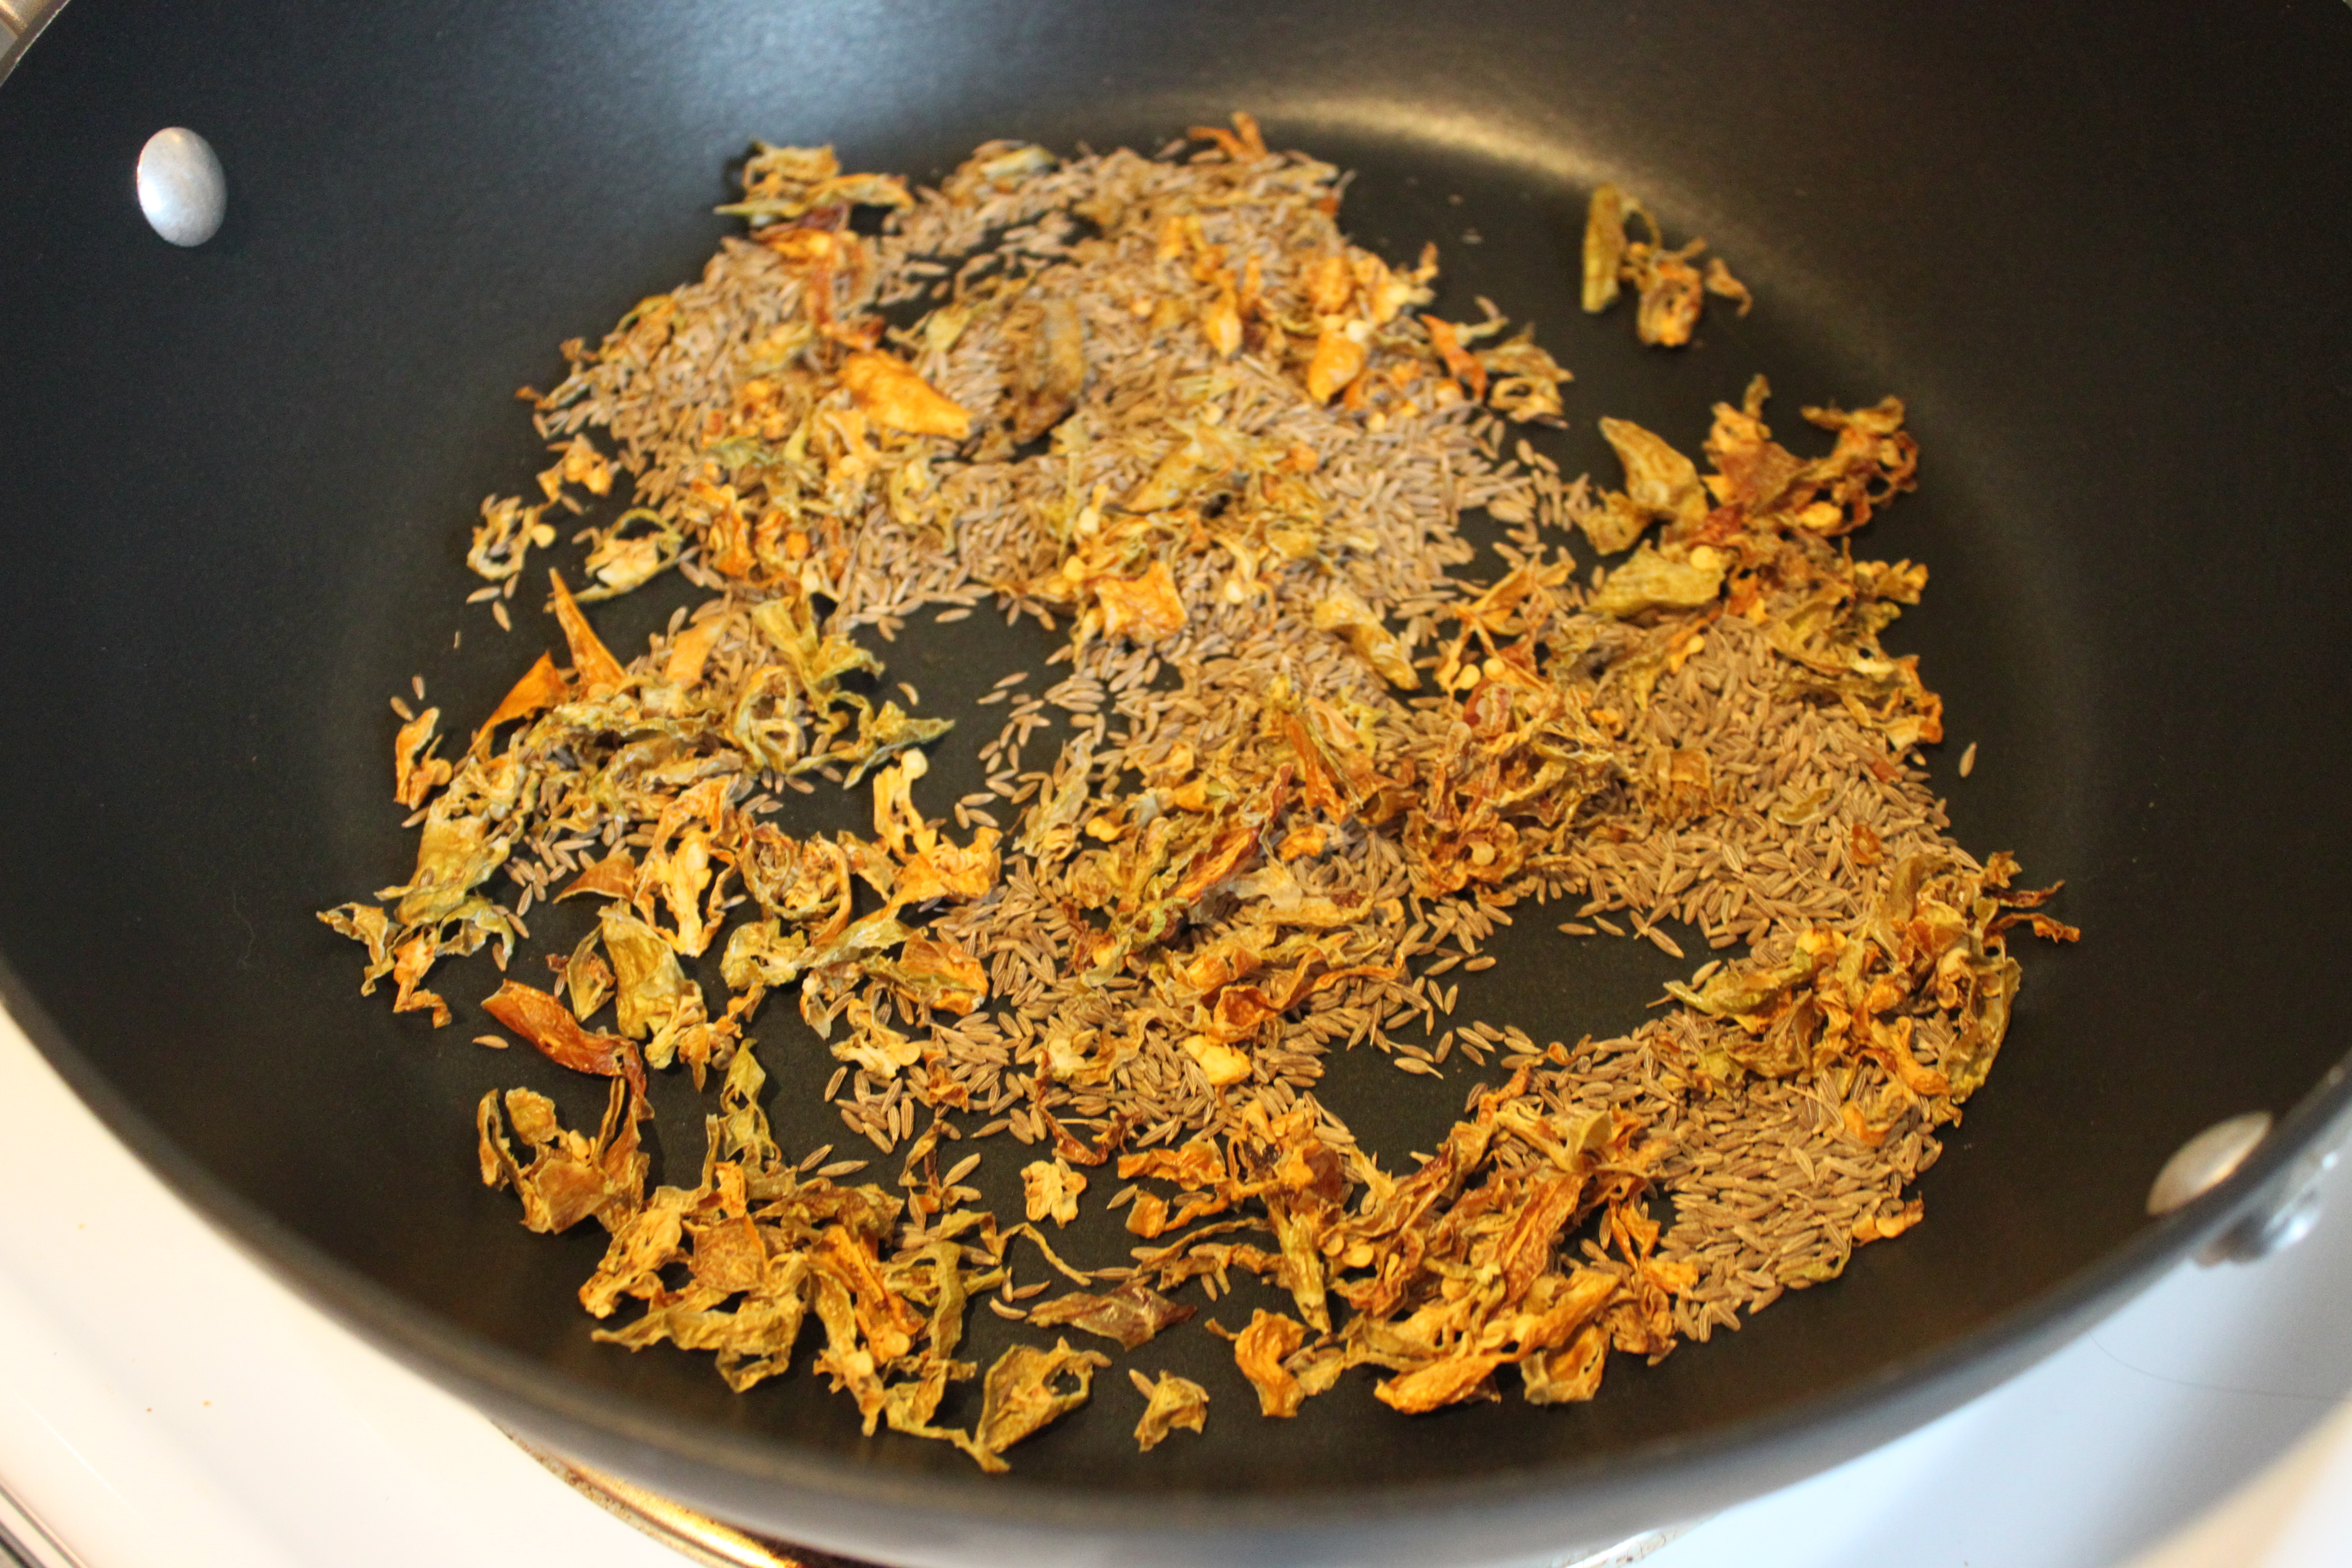
\includegraphics[height=0.3\textwidth]{./../figures/datil-sgy}
%% \end{center}
%% \caption*{Datil chili peppers and whole cumin seed}
%% \end{figure}
